\pdfoptionpdfminorversion=5
\documentclass[9pt,hyperref={pdfpagelabels=false}]{beamer}

\mode<presentation> {
    \usetheme{HHUD}
    \setbeamercovered{invisible}
}
\usepackage[ngerman]{babel}
\usepackage[utf8x]{inputenc}
\usepackage{times}
\usepackage[T1]{fontenc}
\usepackage{amsmath}
\usepackage{subfigure}
\usepackage{graphicx}
\usepackage{hyperref}
\usepackage{grffile}
\usepackage{xmpmulti}
\usepackage{multicol}
\usepackage{appendixnumberbeamer}

% background image
\usebackgroundtemplate{
\includegraphics[width=\paperwidth]{fig/background}}
% commands for low and high decoration in frame foot
\newcommand{\footdecorationlow}{\usebackgroundtemplate{
\includegraphics[width=\paperwidth]{fig/background_small}}}
\newcommand{\footdecorationhigh}{\usebackgroundtemplate{
\includegraphics[width=\paperwidth]{fig/background}}}

\AtBeginSection[] {
  \footdecorationhigh
  \begin{frame}<beamer>
    \thispagestyle{empty}
    \frametitle{Outline}
    \vspace{-5mm}
    \tableofcontents[currentsection]
  \end{frame}
  \footdecorationlow
}

\newcommand{\simtd}{$\text{sim}^\text{TD}$}
 
% % % % % % % % % %  CHANGE TOPIC AND AUTHOR INFORMATION HERE % % % % % % % % %
\title[Kurztitel]{Analysis of Buffer Management Policies \\ for Opportunistic Networks}
\author[Kurzautor]{Christopher Probst}
\institute{University of D\"usseldorf, HHU - 2015 SS - Opportunistic and Peer-to-Peer Networks}
\subject{Computer Science}
\date{23.07.2015}
% % % % % % % % % % % % % % % % % % % % % % % % % % % % % % % % % % % % % % % %

\begin{document}

  \footdecorationhigh
  \begin{frame}
    \thispagestyle{empty}
    \titlepage
  \end{frame}
  
  \begin{frame}
    \thispagestyle{empty}
    \frametitle{Outline}
    \vspace{-5mm}
    \tableofcontents
  \end{frame}
  \footdecorationlow

  \section{Introduction}

\begin{frame}
  \frametitle{Motivation}  
  \begin{itemize}
    \item Mobile Web not always available
    \vspace{0.3cm}
    \begin{itemize}
      \item Outside of cities
      \vspace{0.1cm}
      \item Third World countries
      \vspace{0.1cm}
      \item Even in cities, in case of congestion
    \end{itemize}
  \end{itemize}

  \vspace{0.3cm}

  \begin{itemize}
    \item Mobile Web is centralized
    \vspace{0.3cm}
    \begin{itemize}
      \item Single point of failure
      \vspace{0.1cm}
      \item Missing privacy
      \vspace{0.1cm}
      \item Expensive infrastructure => end-users pay
    \end{itemize}
  \end{itemize}
\end{frame}


\begin{frame}
  \frametitle{Possible Solution}  
  \begin{itemize}
    \item Mobile devices communicate with each other
    \vspace{0.3cm}
    \begin{itemize}
      \item WiFi, Bluetooth, IR, NFC, etc.
      \vspace{0.1cm}
      \item Range and bandwidth determined by interface type
      \vspace{0.1cm}
      \item Independent of Mobile Web
    \end{itemize}    

    \vspace{0.3cm}

    \item Message delivery
    \vspace{0.3cm}
    \begin{itemize}
      \item Hop-by-hop routing
      \vspace{0.1cm}
      \item Indeterministic, churn, overhead
      \vspace{0.1cm}
      \item More anonymous than Mobile Web
    \end{itemize} 
  \end{itemize}



\end{frame}


\begin{frame}
  \frametitle{Challenges}  

  \begin{itemize}  
    \item Routing Protocol
    \vspace{0.3cm}
    \begin{itemize}
      \item Network topology constantly changing
      \vspace{0.1cm}
      \item Origin and destination might be isolated
      \vspace{0.1cm}
      \item Node selection for routing
      \vspace{0.1cm}
      \item Different routing strategies      
      \begin{itemize}
        \item Epidemic (used for evaluation)
        \vspace{0.1cm}
        \item PRoPHET
        \vspace{0.1cm}
        \item etc.
      \end{itemize}    
    \end{itemize}    
  \end{itemize}

  \vspace{0.3cm}

  \begin{itemize}  
    \item Buffer Management
    \vspace{0.3cm}
    \begin{itemize}
      \item Queue policy: Buffers messages in send queue
      \vspace{0.1cm}
      \item Drop policy: Drops messages, if queue exhausted
      \vspace{0.1cm}
      \item Effect on routing performance ?
    \end{itemize} 
  \end{itemize}

\end{frame}



  \section{Routing in Opportunistic Networks}


\begin{frame}
  \frametitle{Used Routing Protocol}
  \begin{itemize}
    \item Epidemic
    \vspace{0.3cm}
    \begin{itemize}
      \item Basically flooding
      \vspace{0.1cm}
      \item High delivery probability + overhead
      \vspace{0.1cm}
      \item Exchange summary vectors with nearby nodes
      \vspace{0.1cm}
      \item Transmit missing messages and buffer
      \begin{itemize}
      	\item Based on queue policy
      \end{itemize}
      \vspace{0.1cm}
      \item Drop messages if congested
      \begin{itemize}
      	\item Based on drop policy
      \end{itemize}
      \vspace{0.1cm}
      \item Routing performance inherently based on Buffer Management
      \begin{itemize}
      	\item Good fit for first study
      \end{itemize}
    \end{itemize}
  \end{itemize}
\end{frame}



\begin{frame}
  \frametitle{Other Routing Protocols}
  \begin{itemize}
	\item PRoPHET
    \begin{itemize}
      	\item Probability-based
      	\item Overrides queue policy
        \begin{itemize}
          	\item Fallback if probabilities are equal
        \end{itemize}
    \end{itemize}
    \vspace{0.3cm}
    \item First Contact
	\begin{itemize}
      	\item Node-to-node routing
    \end{itemize}
    \vspace{0.3cm}
    \item Direct Delivery
	\begin{itemize}
      	\item Only deliver to destination directly
    \end{itemize}
    \vspace{0.3cm}
    \item etc.
    \vspace{0.3cm}
  \end{itemize}
\end{frame}


\begin{frame}
  \frametitle{Buffer Management Policy}
  \begin{itemize}
    \item \{Queue, Drop\} Policy == Sorting order
    \vspace{0.3cm}
    \item Popular policies
    \begin{itemize}
      \item FIFO - Arrival-time (ascending)
      \item LIFO - Arrival-time (descending)
    \end{itemize}
    \vspace{0.3cm}
    \item Further policies
    \begin{itemize}
      \item Random
      \item Replications (aka Hop-count) (ascending / descending)
      \item Relayed-nodes (ascending / descending)
      \item Time-to-live (ascending / descending)
      \item Message-size (ascending / descending)
    \end{itemize}
    \vspace{0.3cm}
    \item 11 sorting orders per policy
    \begin{itemize}
      \item 121 different combinations
    \end{itemize}
  \end{itemize}
\end{frame}


  \section{Simulation Setup}


\begin{frame}
  \frametitle{Simulation Setup}
  \begin{itemize}
    \item Opportunistic Network Environment (ONE) simulator
    \vspace{0.3cm}
    \item Supports only two queue policies
	\begin{itemize}
      \item Random, FIFO
    \end{itemize}
    \vspace{0.3cm}
    \item Supports only one drop policy
	\begin{itemize}
      \item FIFO
    \end{itemize}
	\vspace{0.2cm}
	\item Inherently single-threaded
	\vspace{0.3cm}
	\item Contribution
	\begin{itemize}
      \item Implementations for all policies
      \item Parallelized by running multiple instances
    \end{itemize}
  \end{itemize}
\end{frame}


\begin{frame}
  \frametitle{Methodology}
  \begin{itemize}
	\item Multiple scenarios and metrics
	\begin{itemize}
      \item Each scenario extends base scenario
      \item 121 runs per simulated scenario
    \end{itemize}
    \vspace{0.3cm}
	\item Four scenarios
    \begin{itemize}
	  \item Simulated
	  \begin{itemize}
		\item Medium Traffic
	    \item Frequent and Medium Traffic
	    \item Frequent, Medium and Demanding Traffic
	  \end{itemize}
      \item Computed
	  \begin{itemize}
	  	\item Composite scenario evaluation
	  \end{itemize}
    \end{itemize}
	\vspace{0.3cm}
    \item Four metrics
    \begin{itemize}
      \item Measured
      \begin{itemize}
		\item Delivery Ratio
	    \item Overhead Factor
	    \item Average Delay
	  \end{itemize}
      \item Computed
      \begin{itemize}
	  	\item Composite
	  \end{itemize}
    \end{itemize}
  \end{itemize}
\end{frame}


\begin{frame}
  \frametitle{Methodology}
  \begin{itemize}
	\item Multiple scenarios and metrics
	\begin{itemize}
      \item Each scenario extends base scenario
      \item 121 runs per simulated scenario
    \end{itemize}
    \vspace{0.3cm}
	\item Four scenarios
    \begin{itemize}
	  \item Simulated
	  \begin{itemize}
		\item Medium Traffic
	    \item Frequent and Medium Traffic
	    \item Frequent, Medium and Demanding Traffic
	  \end{itemize}
      \item Computed
	  \begin{itemize}
	  	\item Composite scenario evaluation
	  \end{itemize}
    \end{itemize}
	\vspace{0.3cm}
    \item Four metrics
    \begin{itemize}
      \item Measured
      \begin{itemize}
		\item Delivery Ratio
	    \item Overhead Factor
	    \item Average Delay
	  \end{itemize}
      \item Computed
      \begin{itemize}
	  	\item Composite
	  \end{itemize}
    \end{itemize}
  \end{itemize}
\end{frame}


  \section{Scenarios}


\begin{frame}
  \frametitle{Base Scenario}
	\begin{table}[!ht]	
		\small
	    \begin{tabular}{ | p{0.6\columnwidth} | p{0.3\columnwidth} | }    
	    \hline
	    Parameter & Value \\ \hline \hline 
	    \hline
	    Simulation time & 12 hours \\ \hline
	    Total Number of Nodes & 126 \\ \hline
	    Total Number of Node Groups & 6 \\ \hline \hline    
	    Routing Protocol & Epidemic \\ \hline
	    Buffer Management Policies & $11 * 11 = 121$ \\ \hline
	    2x Pedestrian Group [Count;~Speed] & 40;~0.5-1.5 m/s  \\ \hline
		1x Car Group [Count;~Speed] & 40;~2.7-13.9 m/s  \\ \hline
		3x Tram Group [Count;~Speed] & 2;~7-10 m/s  \\ \hline \hline
	    Movement Model 1 (M1) & Shortest Path Map based Movement \\ \hline
	    Movement Model 2 (M2) & Map Route Movement \\ \hline    
	    Movement Model Groups [M1;~M2] &  3;~3 \\ \hline
	    Movement Model Buffers [M1;~M2] & 5 MB;~50 MB \\ \hline \hline
	    Interface types & Low-Speed, High-Speed \\ \hline
	    Low-Speed [Range;~Bandwidth] & 10 m;~250 KB/s \\ \hline
	    High-Speed [Range;~Bandwidth] & 1 km;~10 MB/s \\ \hline
	    Groups using Low-Speed & All \\ \hline
	    Groups using High-Speed & 1x Tram Group \\ \hline \hline    
	    \end{tabular}
	\end{table}
\end{frame}


\begin{frame}
  \frametitle{Scenarios}
	\begin{table}[!ht]
		\small
	    \begin{tabular}{ | p{0.6\columnwidth} | p{0.3\columnwidth} | }    
	    \hline
	    Parameter & Value \\ \hline \hline 
	    \hline
	    Message Generators & 1 \\ \hline
	    Message Generator 1 [Interval;~Size] & 25-35 s; 0.5-1 MB \\ \hline 
	    \hline
	    \end{tabular}
	    \caption{Scenario 1}
	\end{table}

	\begin{table}[!ht]
		\small
	    \begin{tabular}{ | p{0.6\columnwidth} | p{0.3\columnwidth} | }    
	    \hline
	    Parameter & Value \\ \hline \hline 
	    \hline
	    Message Generators & 2 \\ \hline
	    Message Generator 1 [Interval;~Size] & 1-5 s; 0.5-2 KB \\ \hline 
	    Message Generator 2 [Interval;~Size] & 25-35 s; 64-512 KB \\ \hline 
	    \hline
	    \end{tabular}
	    \caption{Scenario 2}
	\end{table}

	\begin{table}[!ht]
		\small	
	    \begin{tabular}{ | p{0.6\columnwidth} | p{0.3\columnwidth} | }    
	    \hline
	    Parameter & Value \\ \hline \hline 
	    \hline
	    Message Generators & 3 \\ \hline
	    Message Generator 1 [Interval;~Size] & 1-5 s; 0.5-2 KB \\ \hline 
	    Message Generator 2 [Interval;~Size] & 25-35 s; 64-512 KB \\ \hline 
	    Message Generator 3 [Interval;~Size] & 60-120 s; 1-5 MB \\ \hline 
	    \hline
	    \end{tabular}
	    \caption{Scenario 3}
	\end{table}
\end{frame}


  \section{Evaluation}

\begin{frame}
  \frametitle{Scenario 1 - Delivery Ratio}
  \begin{center}
   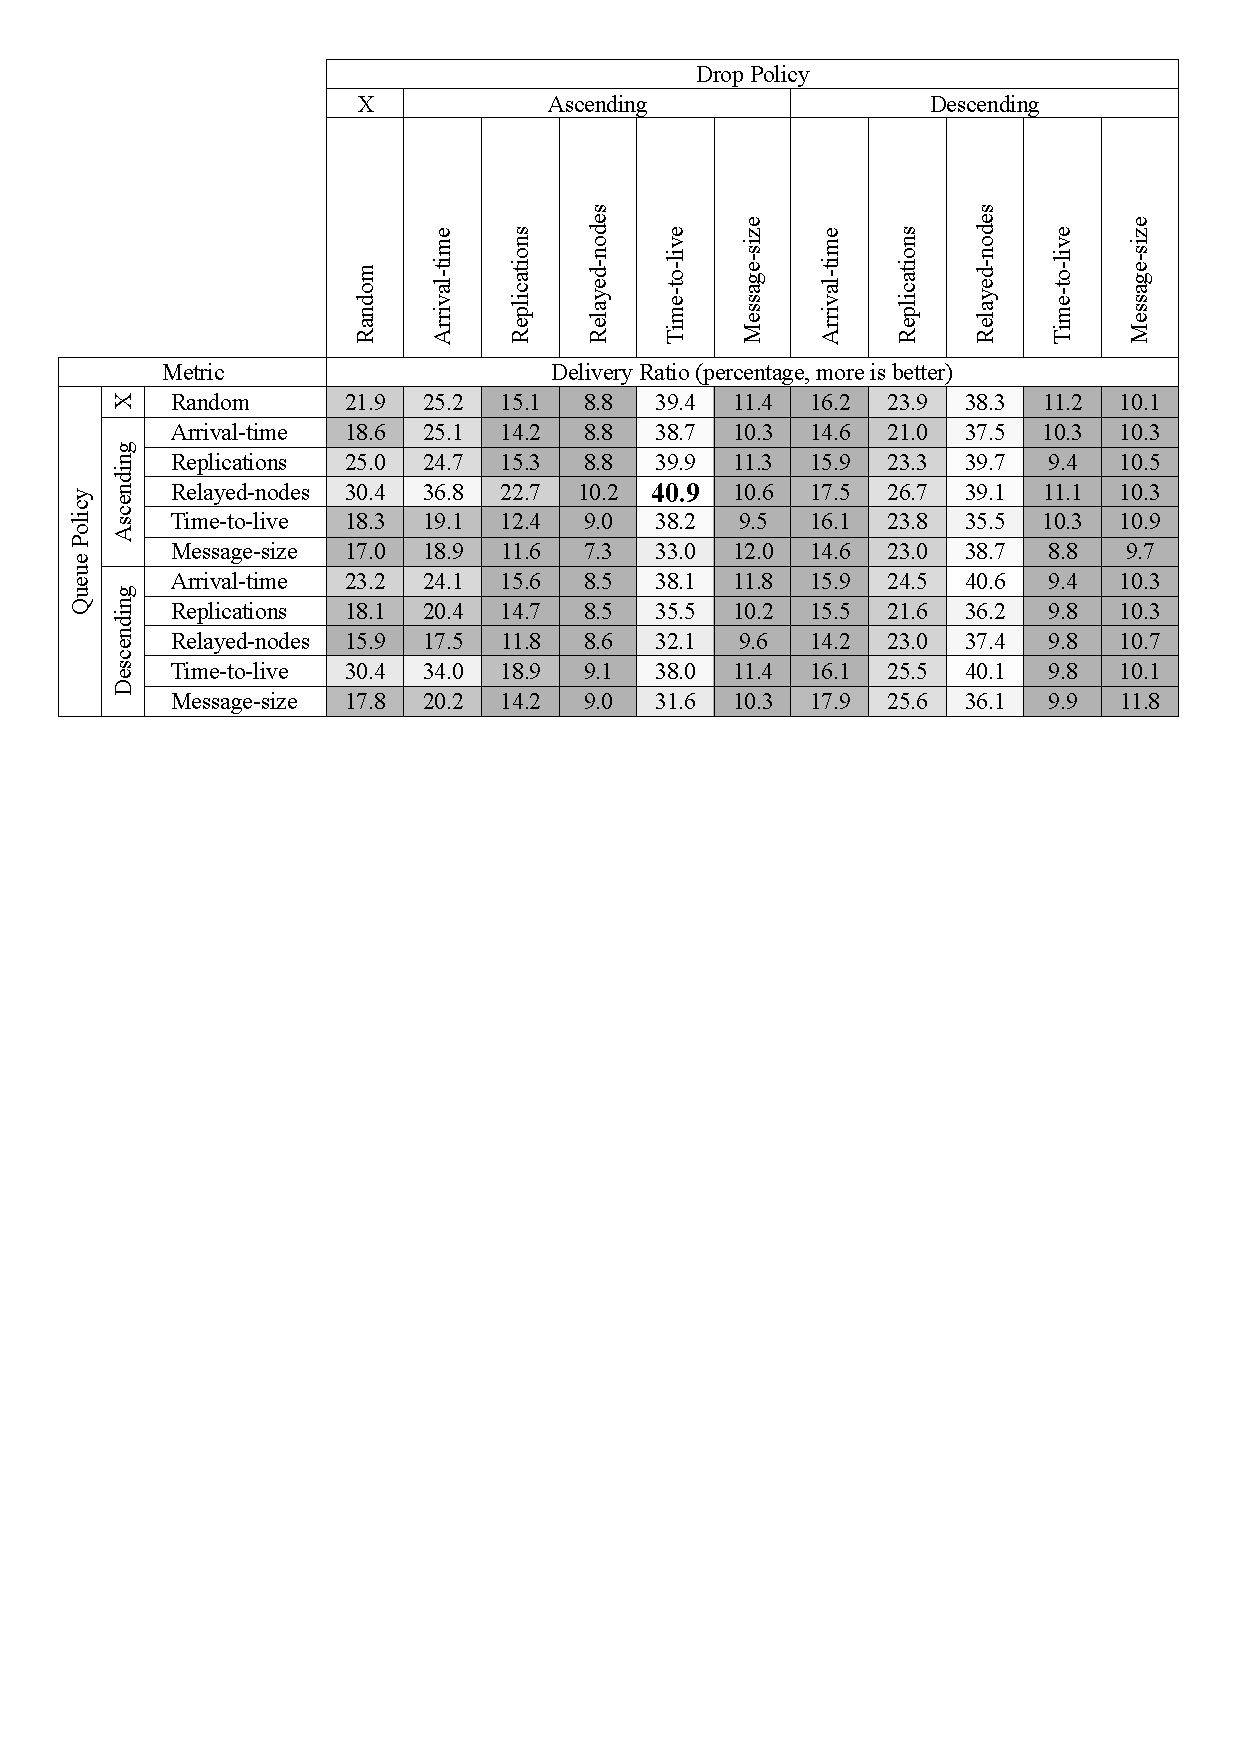
\includegraphics[width=1.0\textwidth]{fig/tables/scenario1_part1.pdf}
  \end{center}
\end{frame}

\begin{frame}
  \frametitle{Scenario 1 - Overhead Factor}
  \begin{center}
   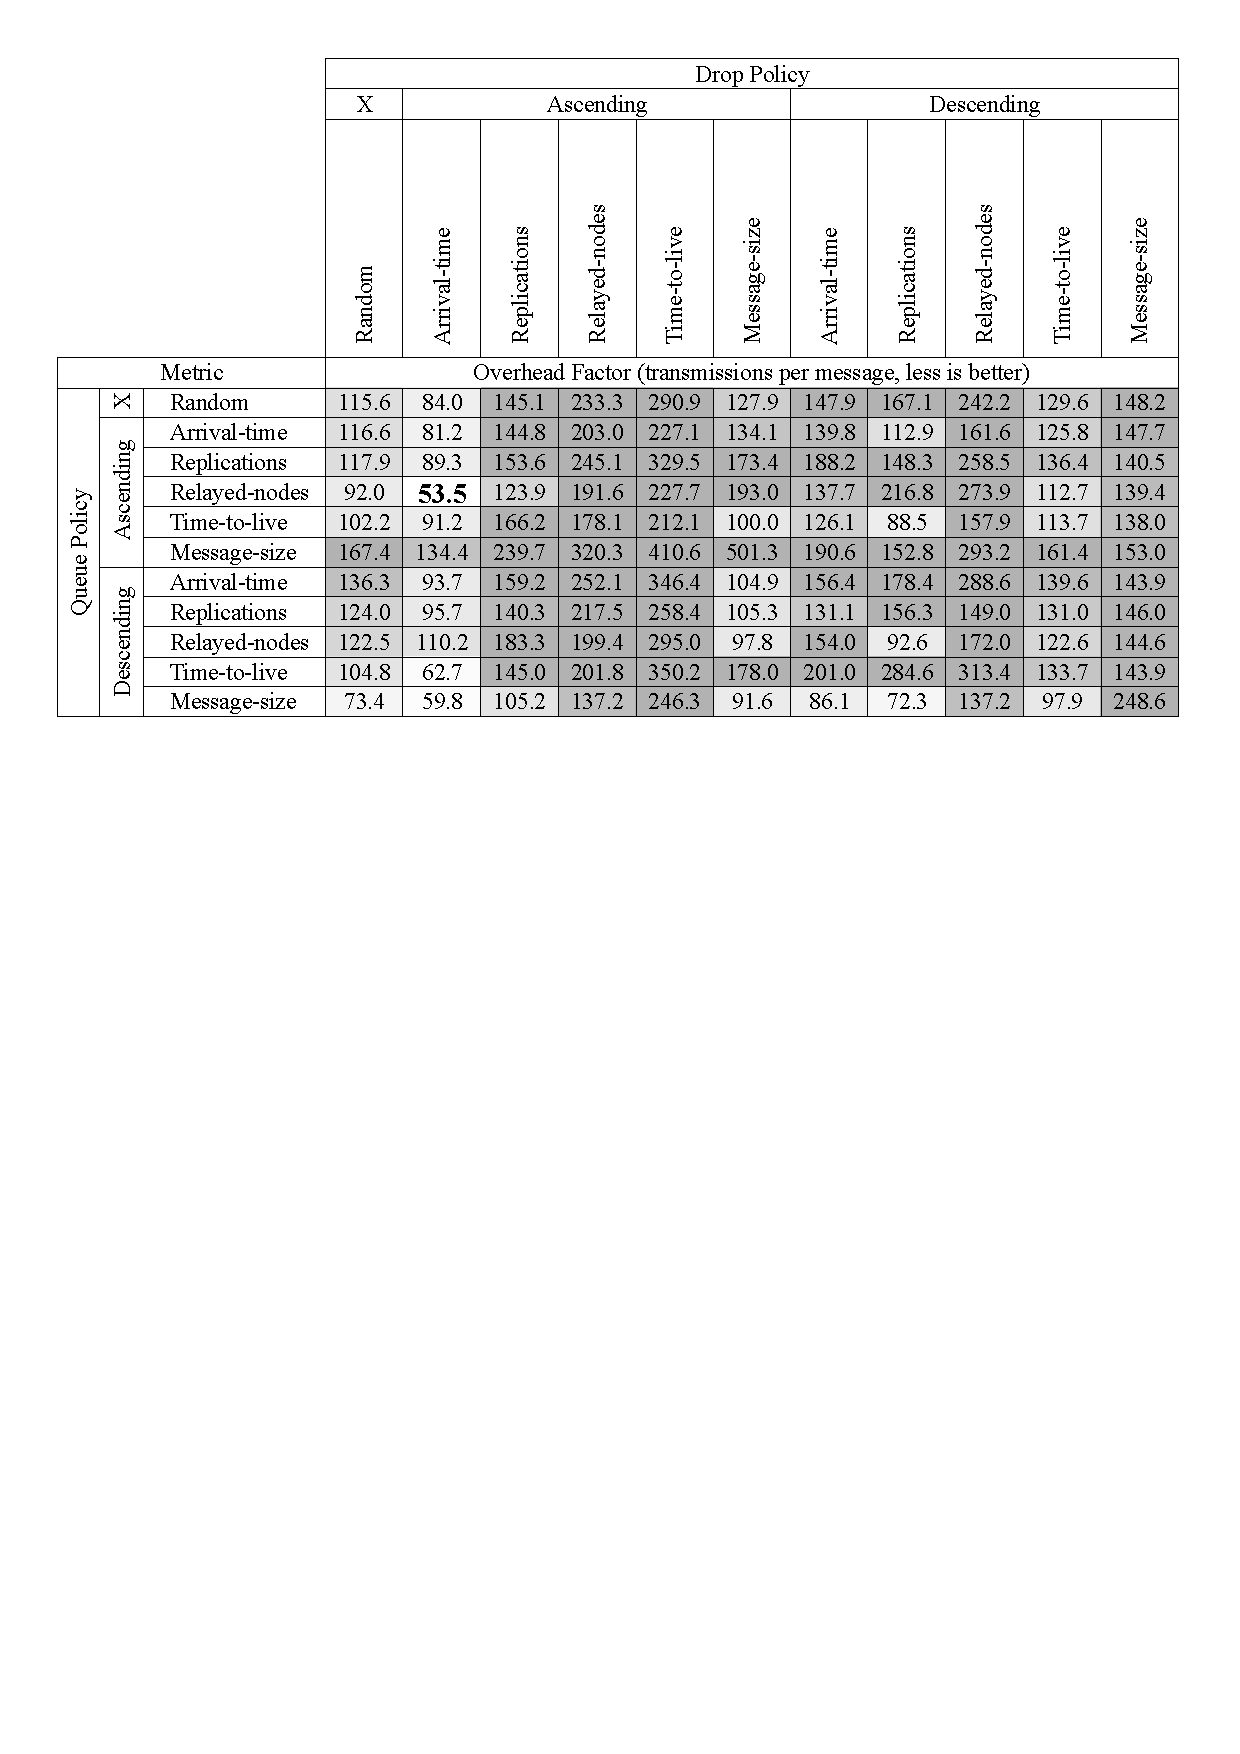
\includegraphics[width=1.0\textwidth]{fig/tables/scenario1_part2.pdf}
  \end{center}
\end{frame}

\begin{frame}
  \frametitle{Scenario 1 - Average Delay}
  \begin{center}
   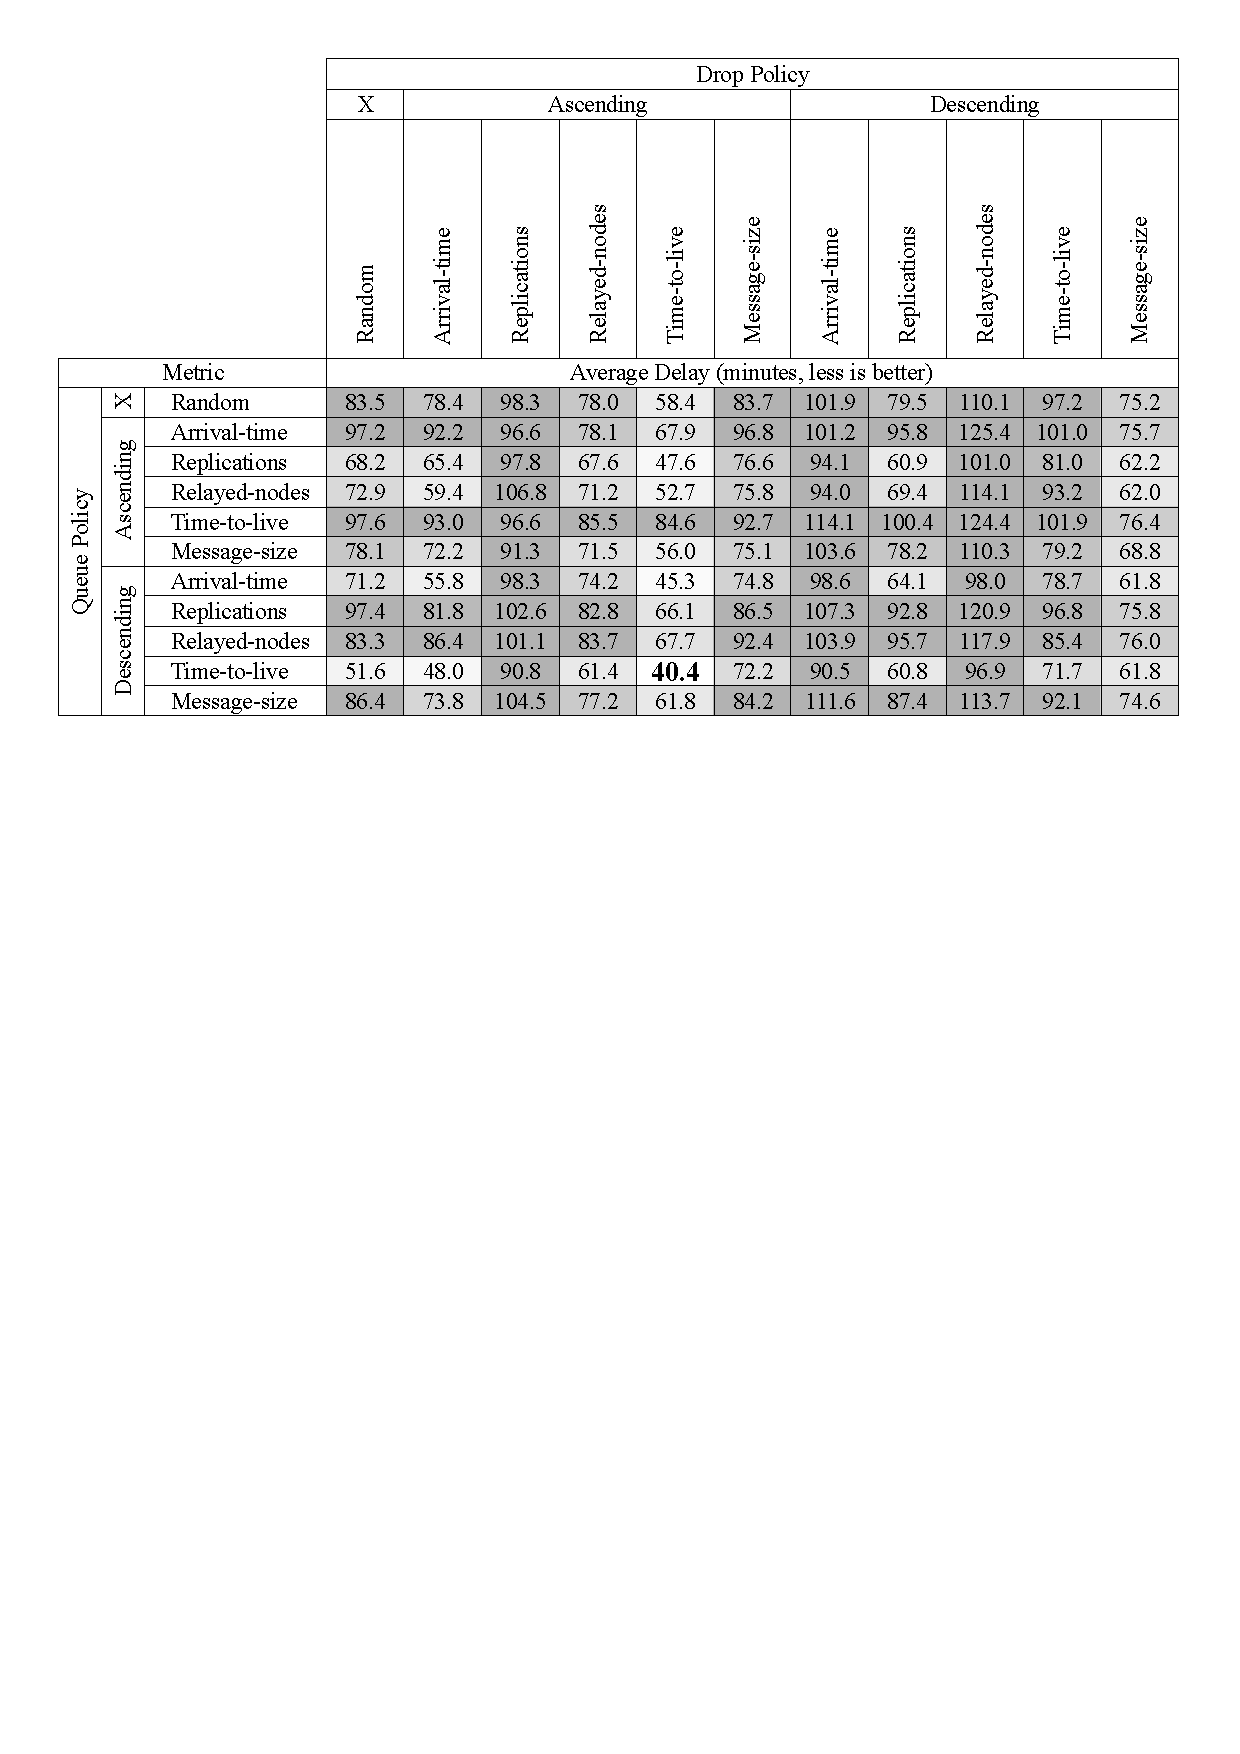
\includegraphics[width=1.0\textwidth]{fig/tables/scenario1_part3.pdf}
  \end{center}
\end{frame}

\begin{frame}
  \frametitle{Scenario 1 - Composite}
  \begin{center}
   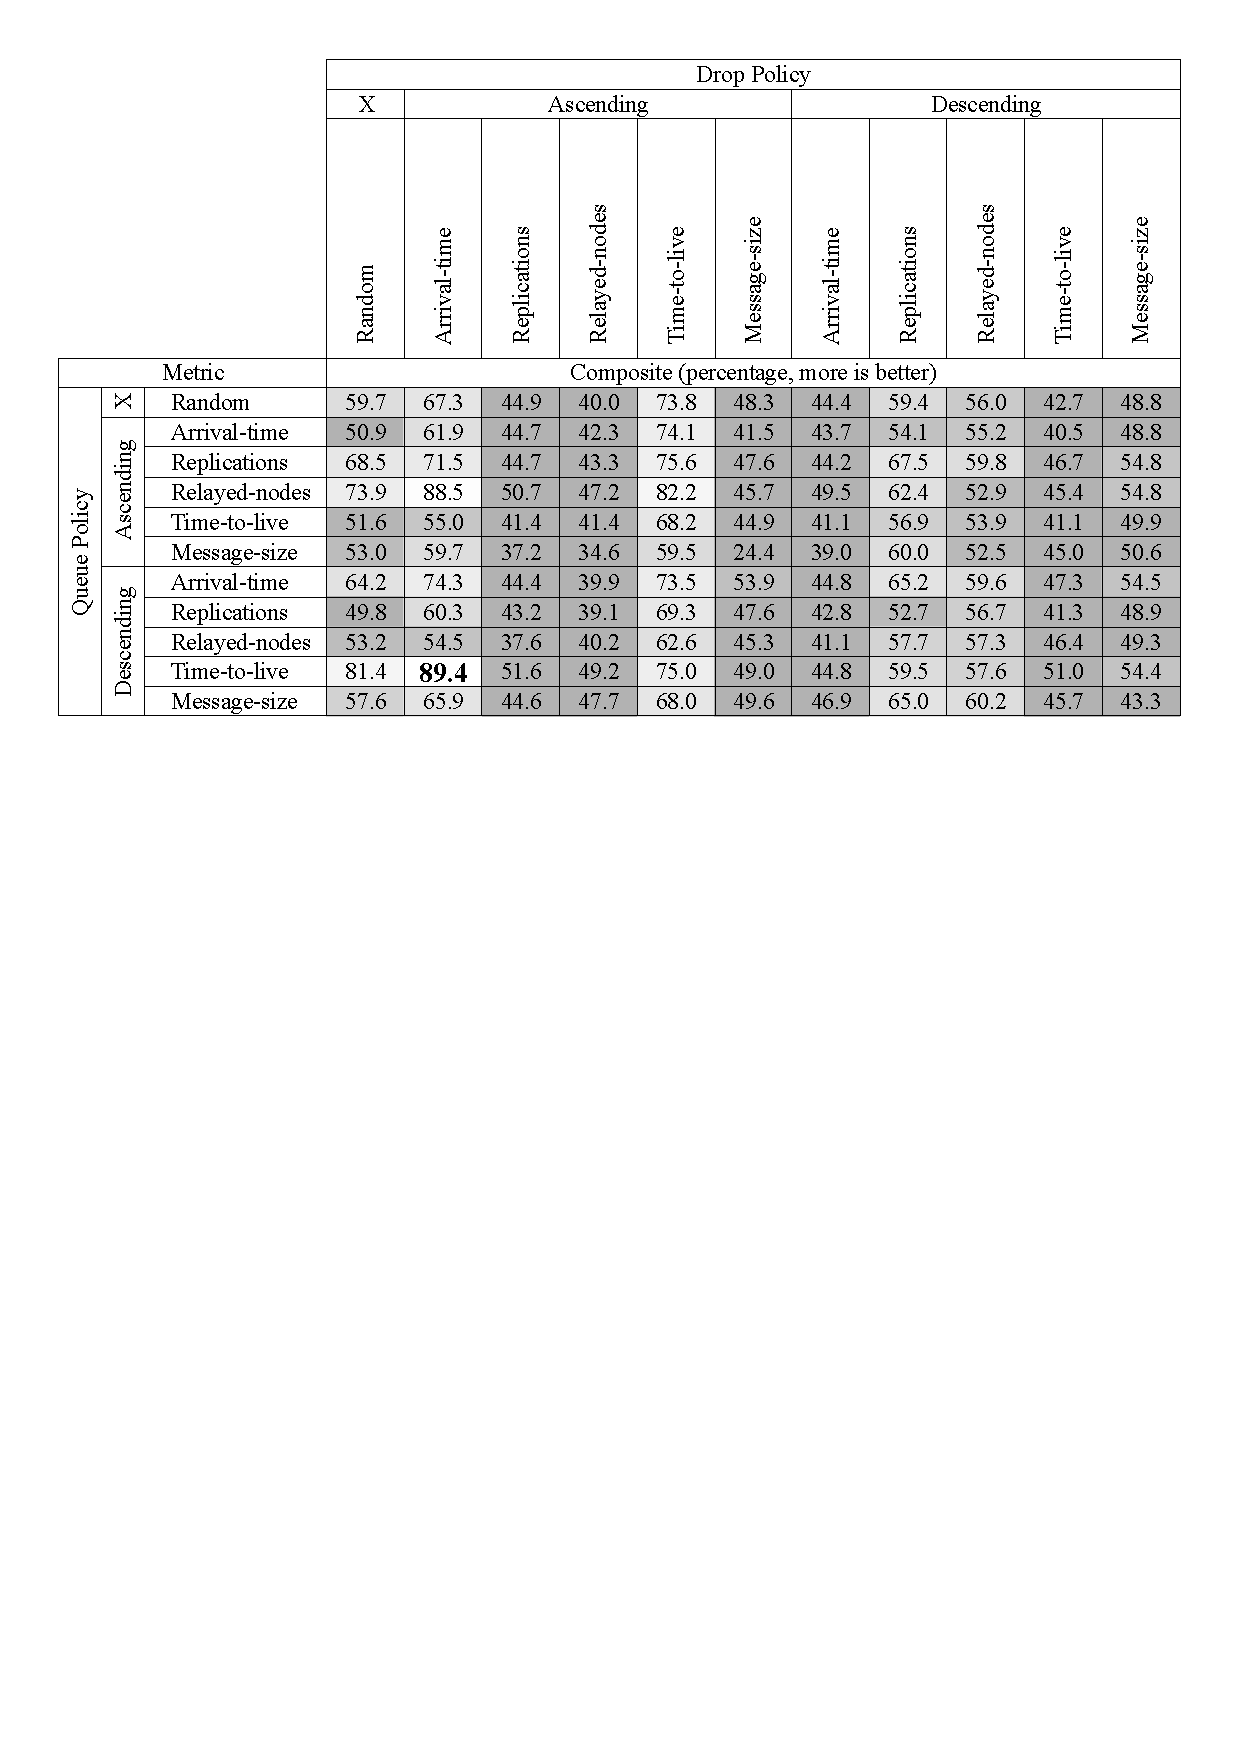
\includegraphics[width=1.0\textwidth]{fig/tables/scenario1_part4.pdf}
  \end{center}
\end{frame}




\begin{frame}
  \frametitle{Scenario 3 - Delivery Ratio}
  \begin{center}
   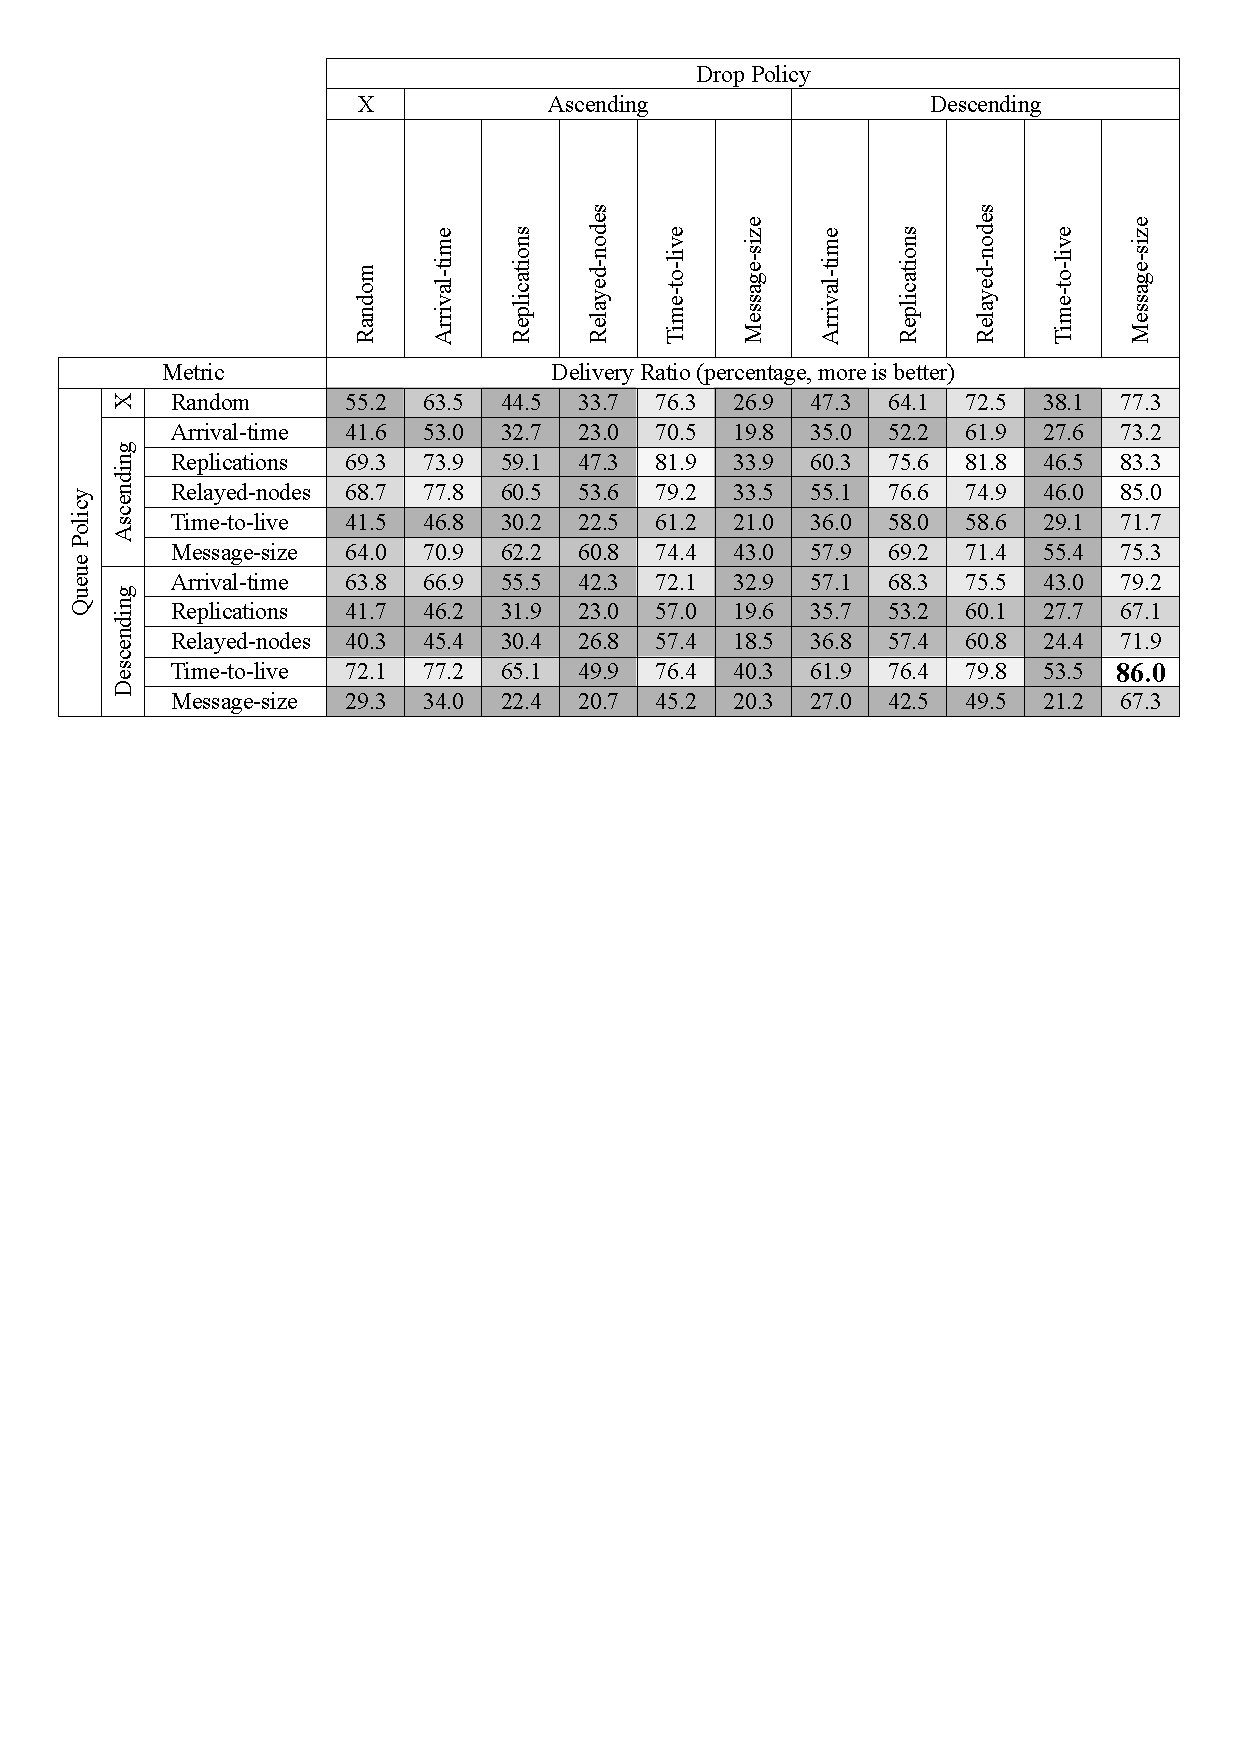
\includegraphics[width=1.0\textwidth]{fig/tables/scenario3_part1.pdf}
  \end{center}
\end{frame}

\begin{frame}
  \frametitle{Scenario 3 - Overhead Factor}
  \begin{center}
   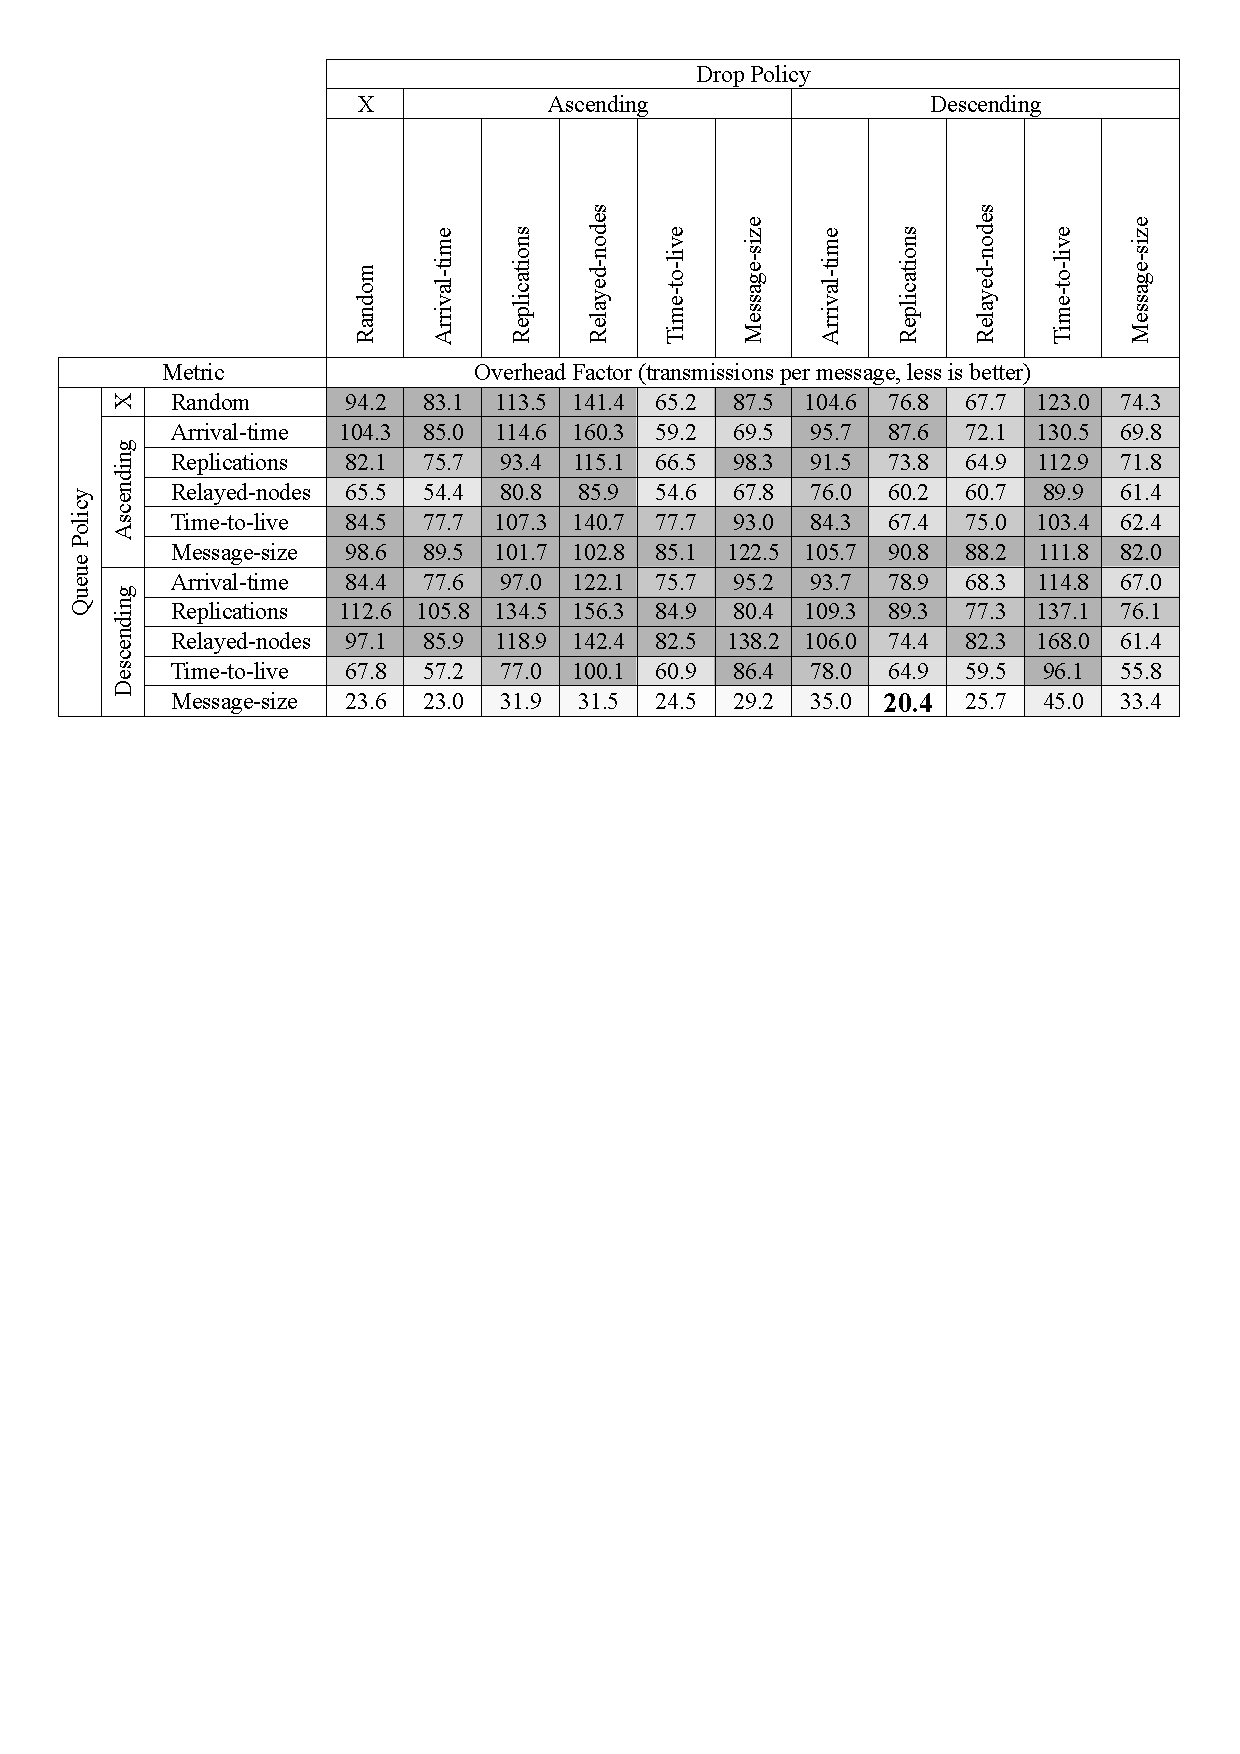
\includegraphics[width=1.0\textwidth]{fig/tables/scenario3_part2.pdf}
  \end{center}
\end{frame}

\begin{frame}
  \frametitle{Scenario 3 - Average Delay}
  \begin{center}
   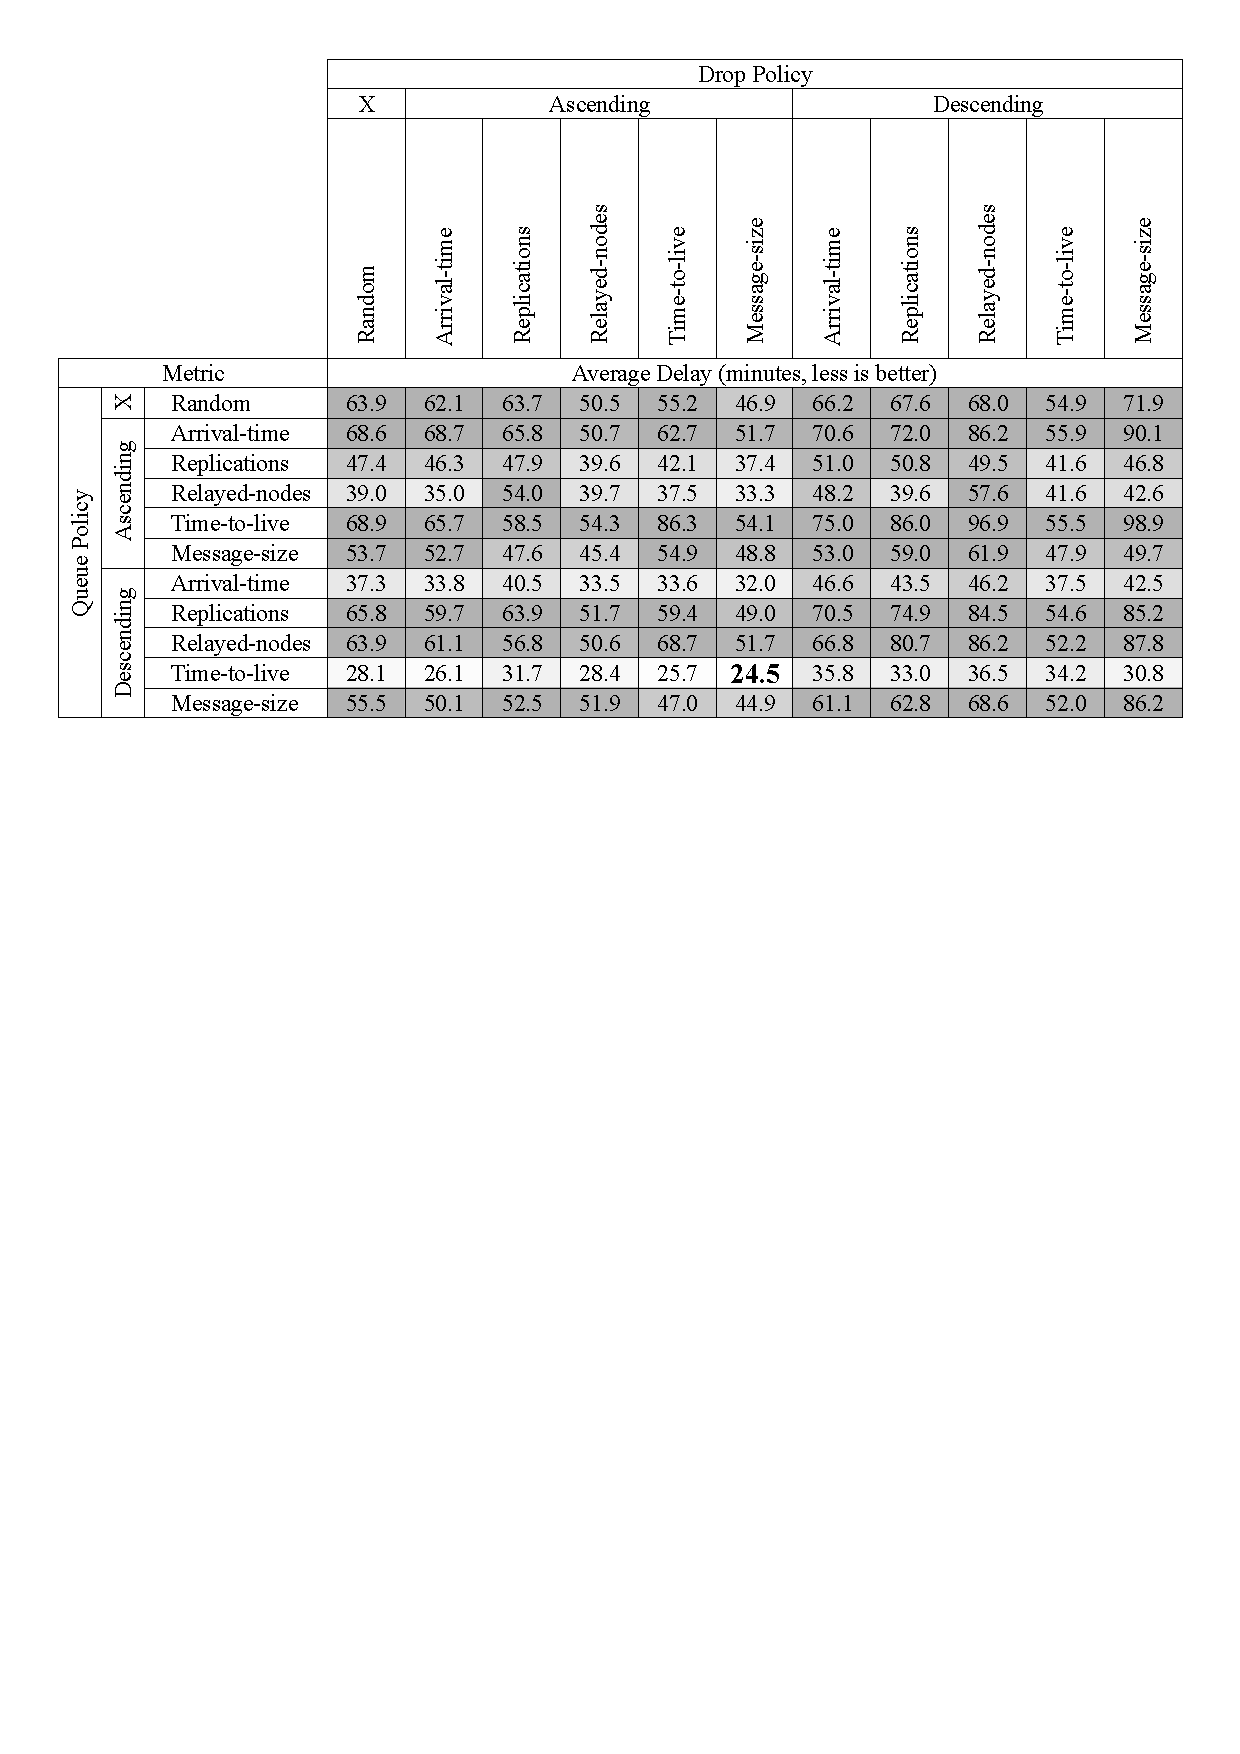
\includegraphics[width=1.0\textwidth]{fig/tables/scenario3_part3.pdf}
  \end{center}
\end{frame}

\begin{frame}
  \frametitle{Scenario 3 - Composite}
  \begin{center}
   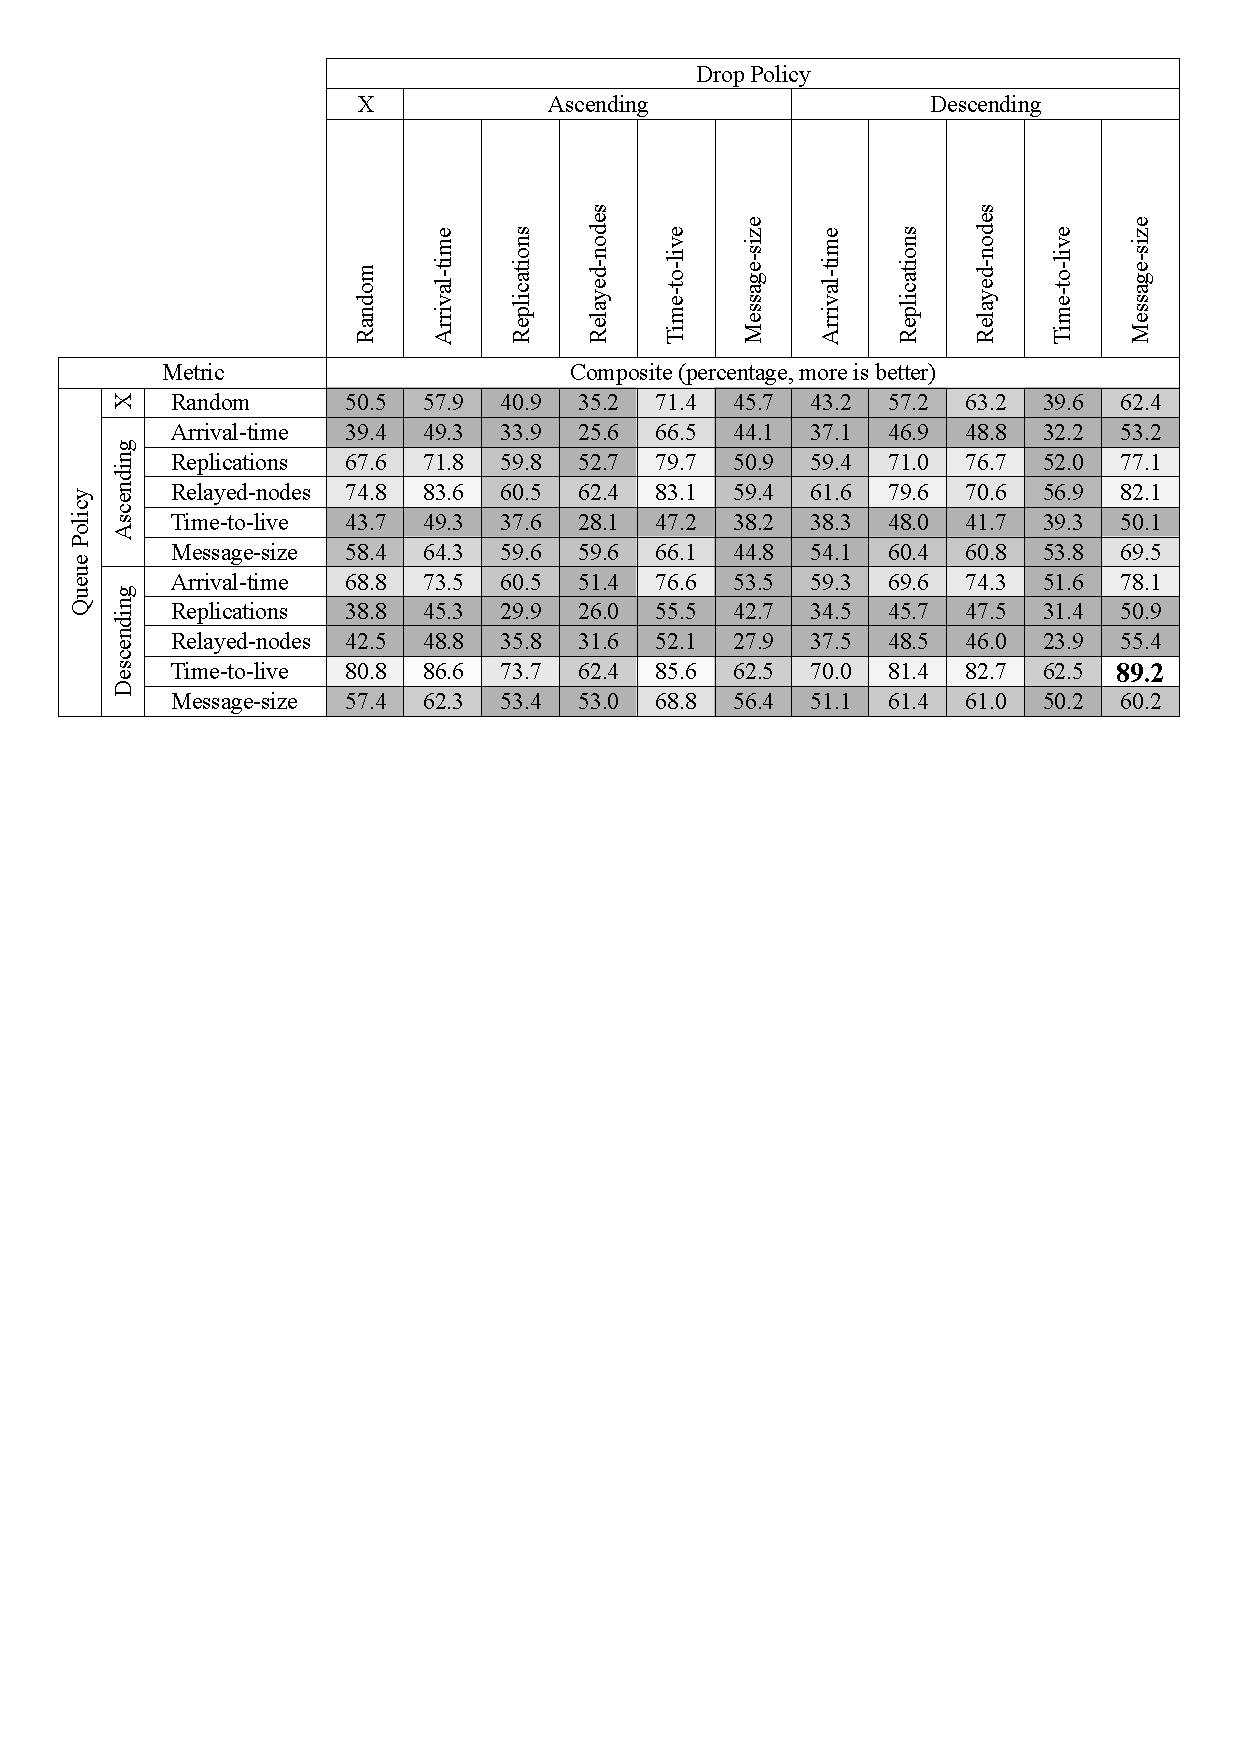
\includegraphics[width=1.0\textwidth]{fig/tables/scenario3_part4.pdf}
  \end{center}
\end{frame}




\begin{frame}
  \frametitle{Composite Scenario Evaluation - Delivery Ratio}
  \begin{center}
   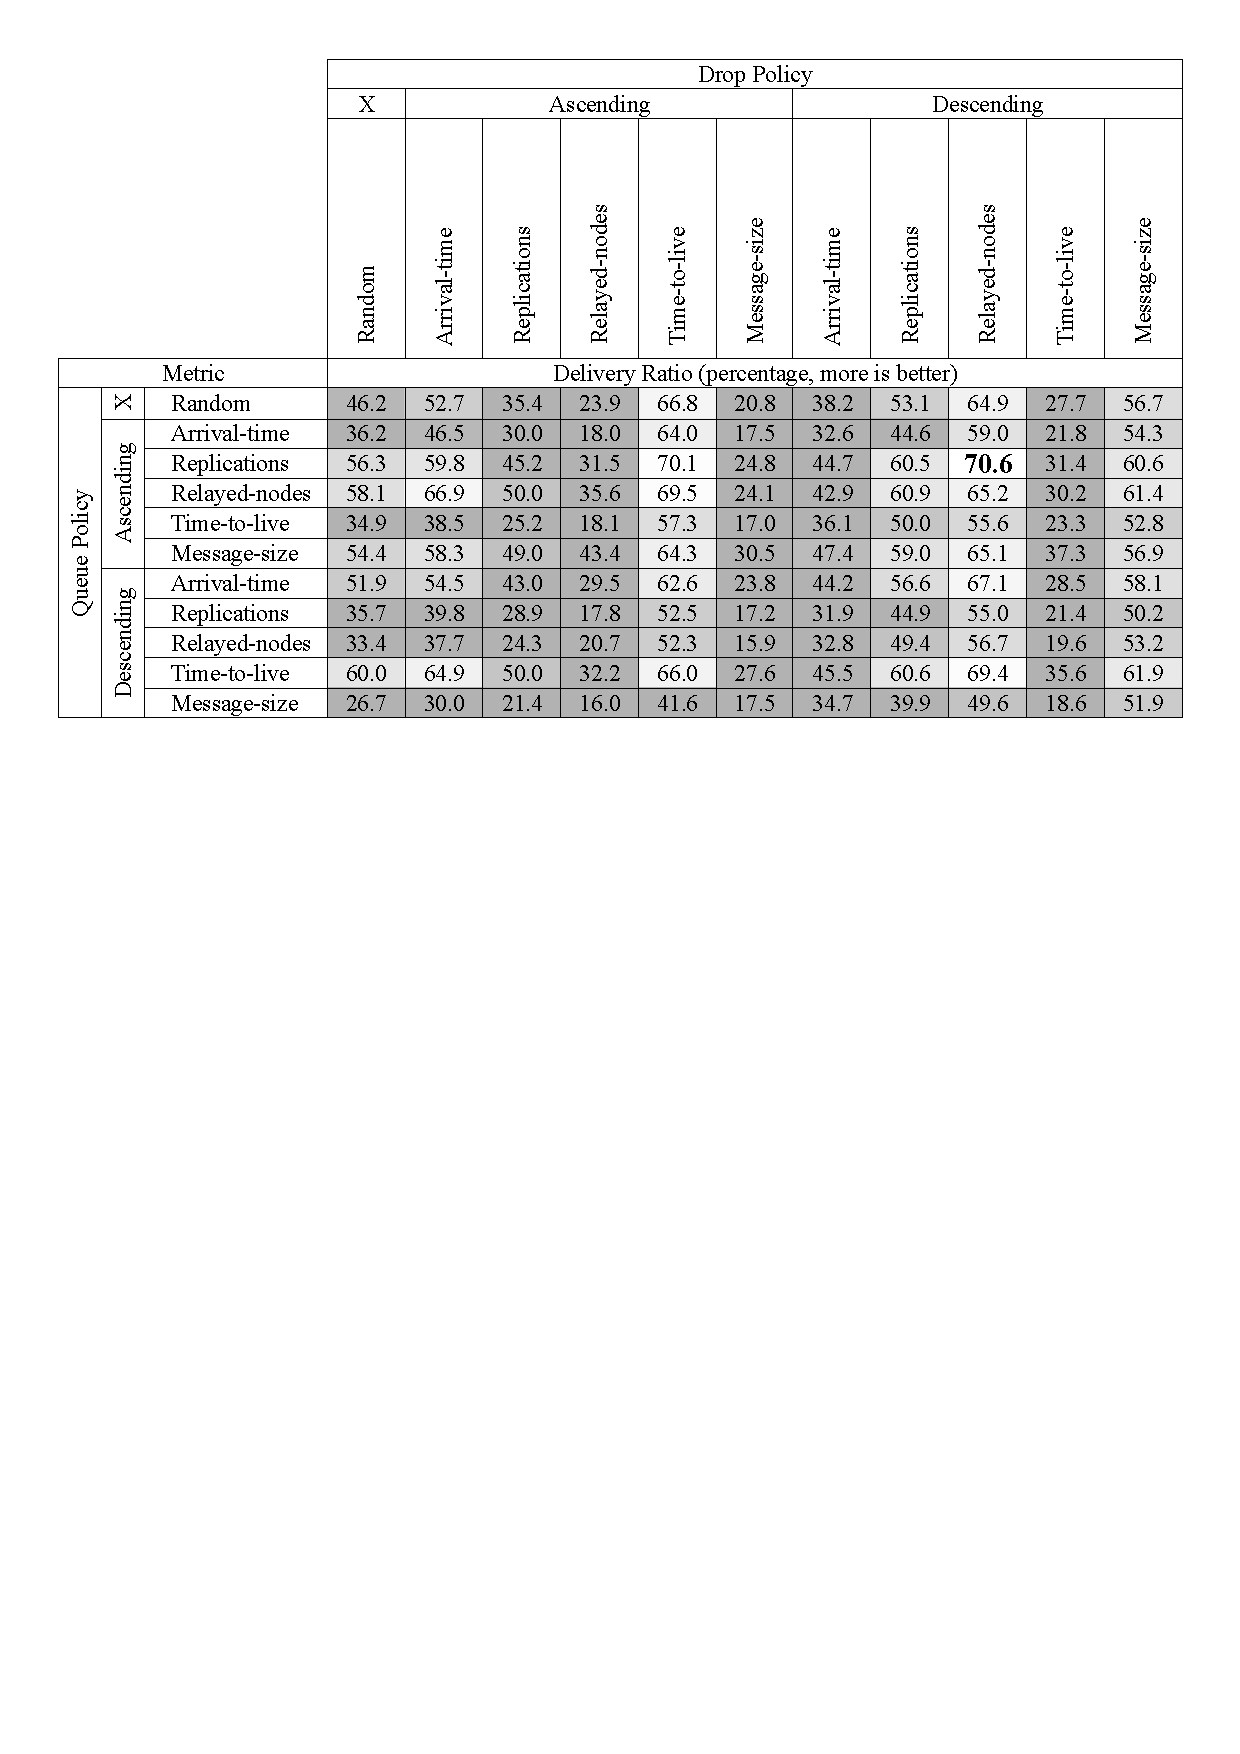
\includegraphics[width=1.0\textwidth]{fig/tables/scenario4_part1.pdf}
  \end{center}
\end{frame}

\begin{frame}
  \frametitle{Composite Scenario Evaluation - Overhead Factor}
  \begin{center}
   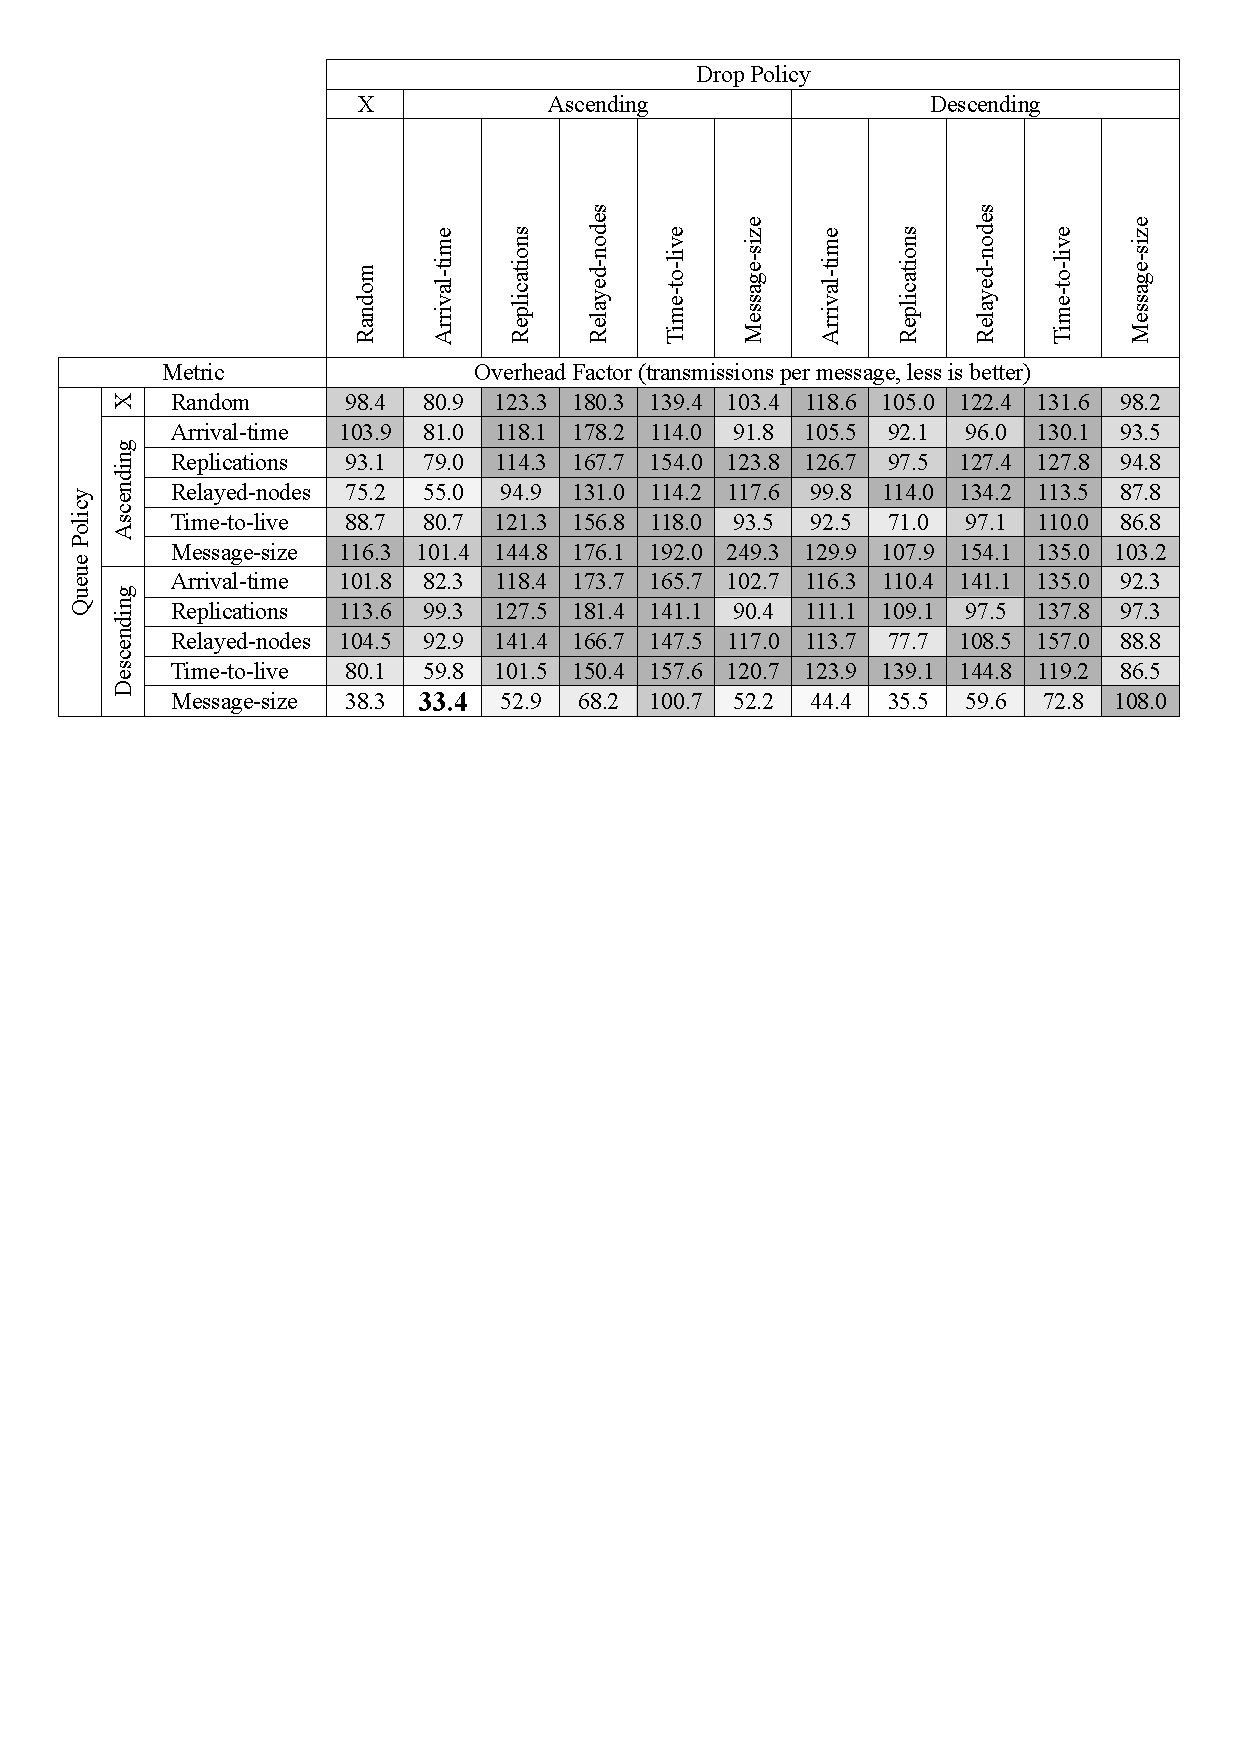
\includegraphics[width=1.0\textwidth]{fig/tables/scenario4_part2.pdf}
  \end{center}
\end{frame}

\begin{frame}
  \frametitle{Composite Scenario Evaluation - Average Delay}
  \begin{center}
   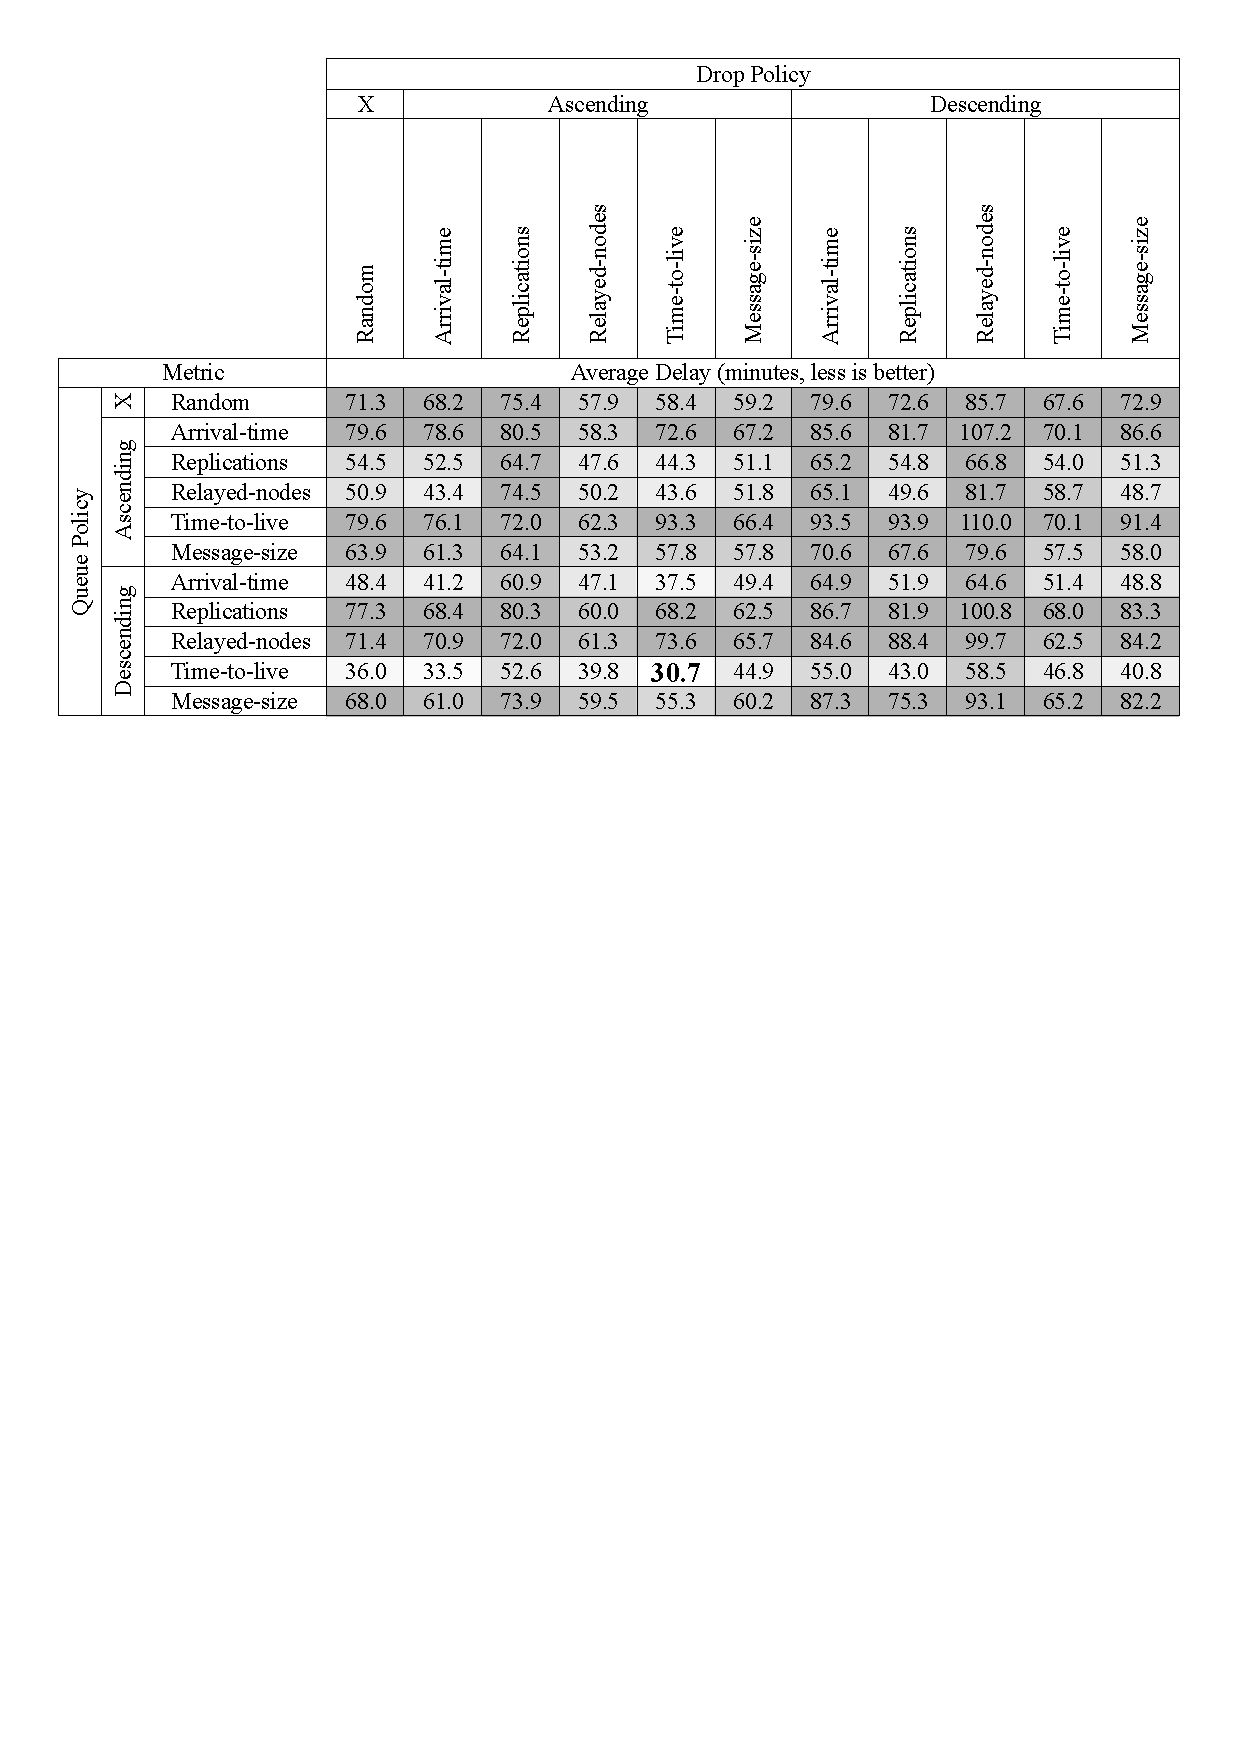
\includegraphics[width=1.0\textwidth]{fig/tables/scenario4_part3.pdf}
  \end{center}
\end{frame}

\begin{frame}
  \frametitle{Composite Scenario Evaluation - Composite}
  \begin{center}
   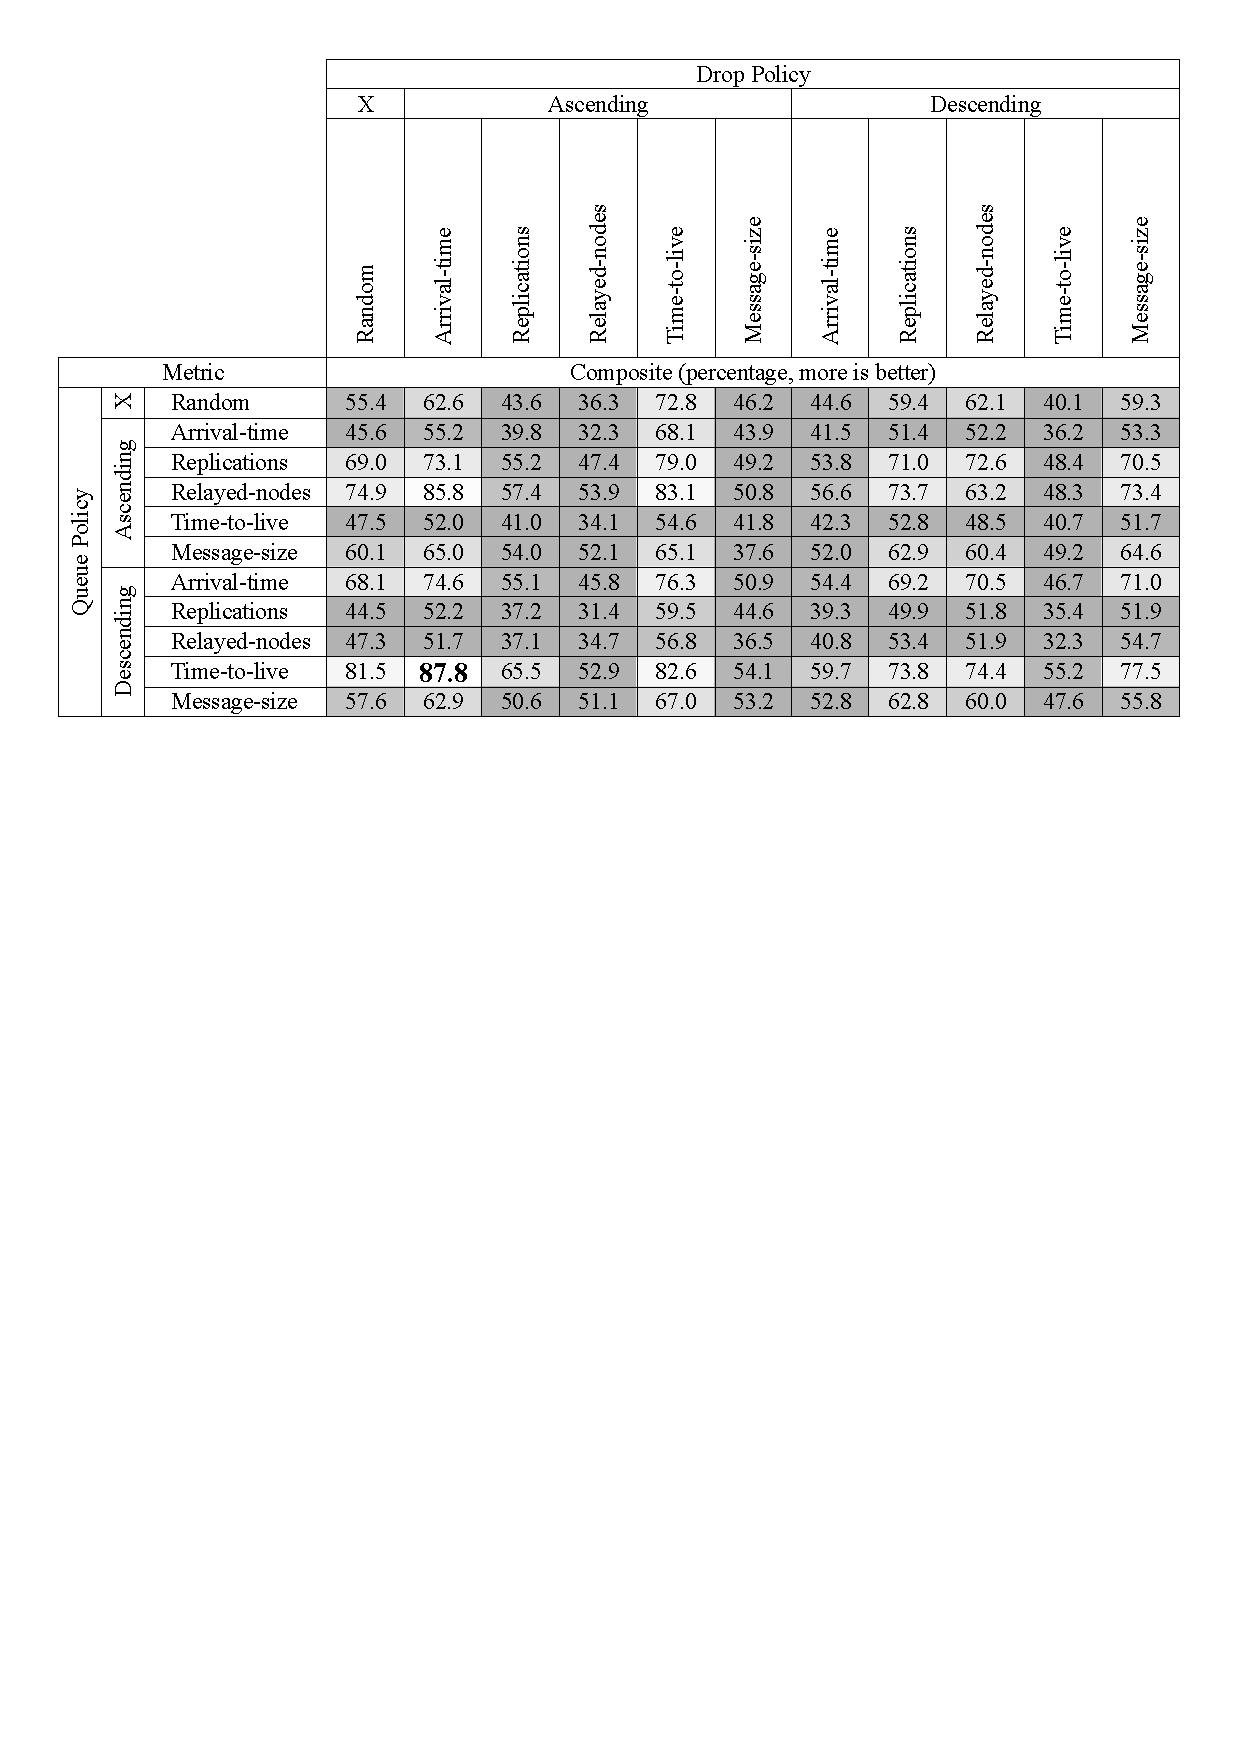
\includegraphics[width=1.0\textwidth]{fig/tables/scenario4_part4.pdf}
  \end{center}
\end{frame}

  \section{Conclusion}

\begin{frame}
  \frametitle{Conclusion}
  \begin{itemize}  
    \item Differently sized messages influence each other
    \vspace{0.3cm}
    \item Epidemic routing performance depends on \{queue, drop\} policy
    \vspace{0.3cm}
    \item Each metrics has other characteristics
    \begin{itemize} 
      \item But: A few policies are preferable on average
    \end{itemize}   
  \end{itemize}		
\end{frame}


\begin{frame}
  \frametitle{Future Work}
  \begin{itemize}
	  \item More scenarios
    \vspace{0.3cm}
    \item More metrics
	  \vspace{0.3cm}	  
	  \item More routing protocols
    \vspace{0.3cm}
    \item More \{queue, drop\} policies    
  \end{itemize}		
\end{frame}

  \appendix

  \begin{frame}
  \frametitle{Scenario 2 - Delivery Ratio}
  \begin{center}
   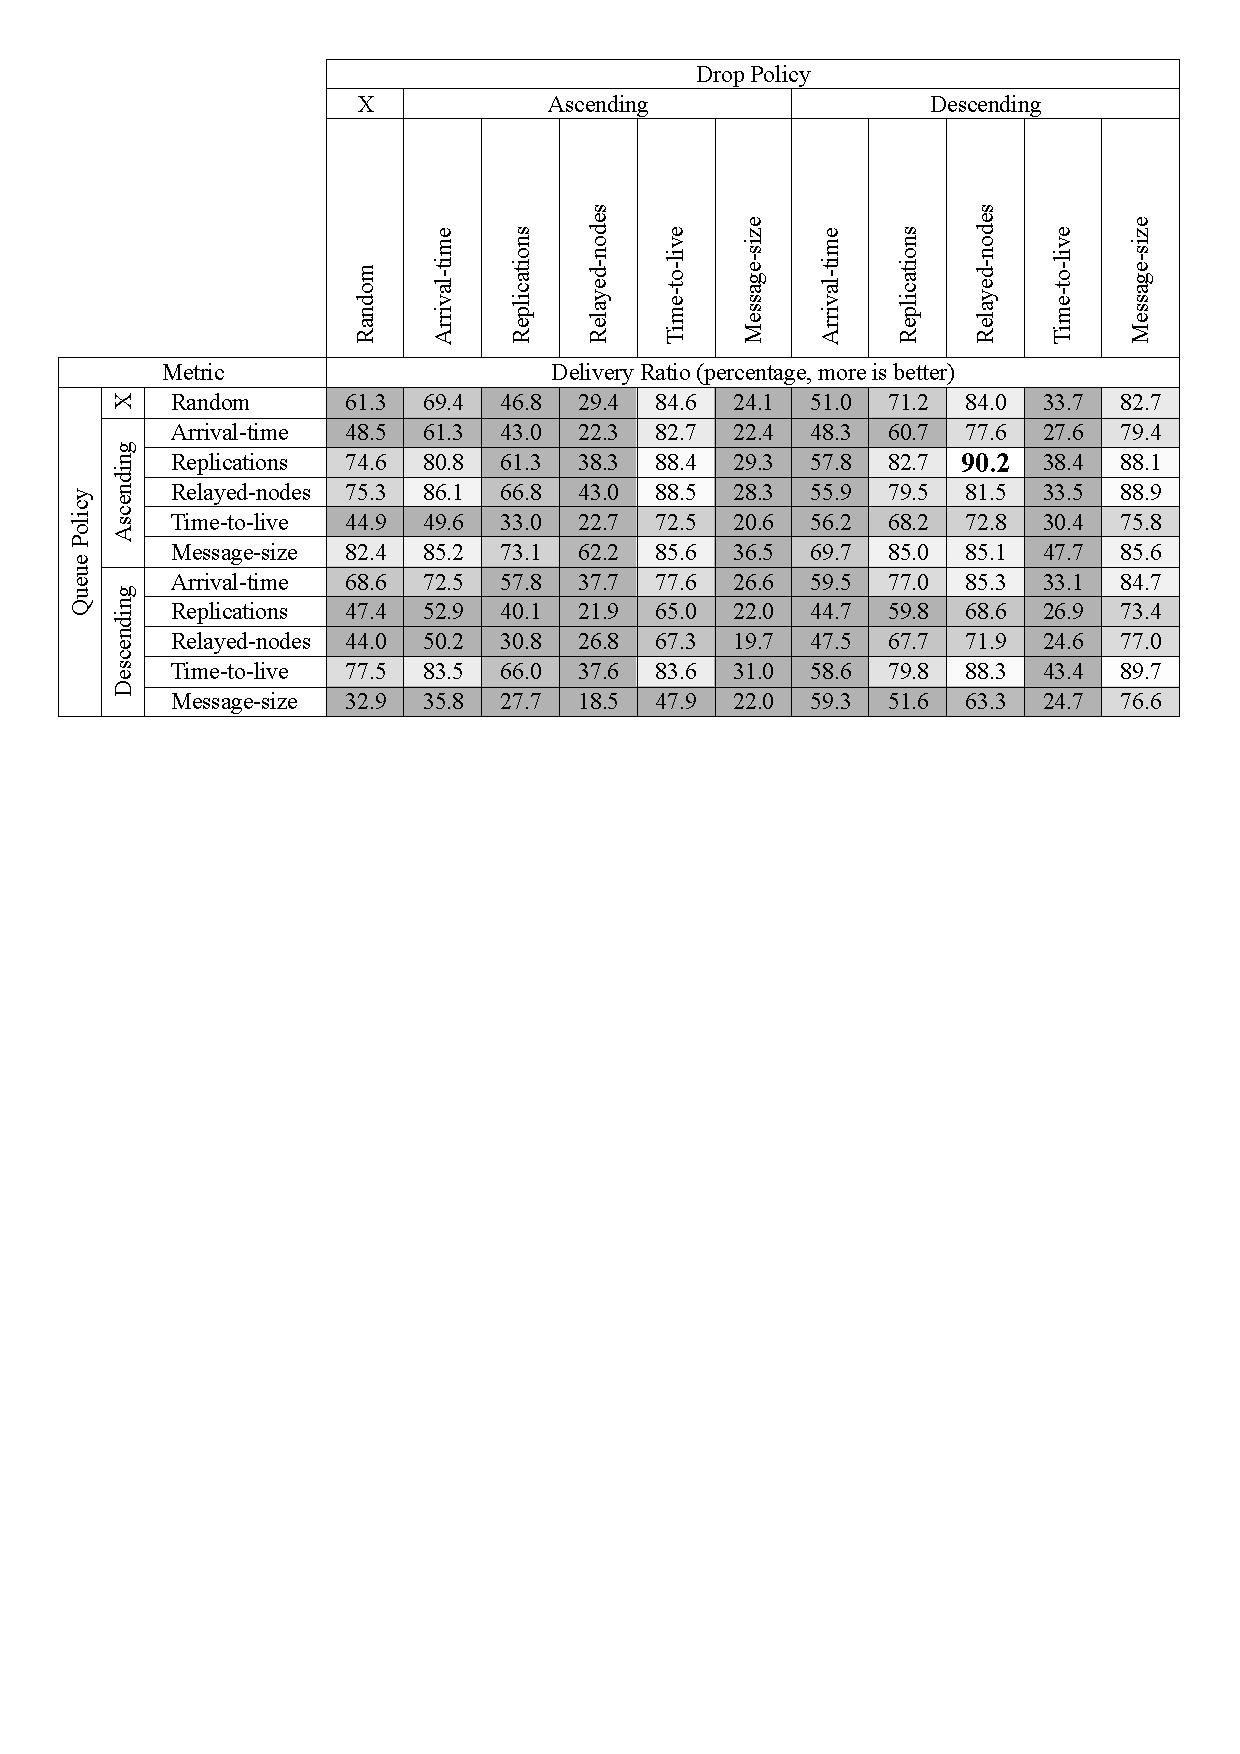
\includegraphics[width=1.0\textwidth]{fig/tables/scenario2_part1.pdf}
  \end{center}
\end{frame}

\begin{frame}
  \frametitle{Scenario 2 - Overhead Factor}
  \begin{center}
   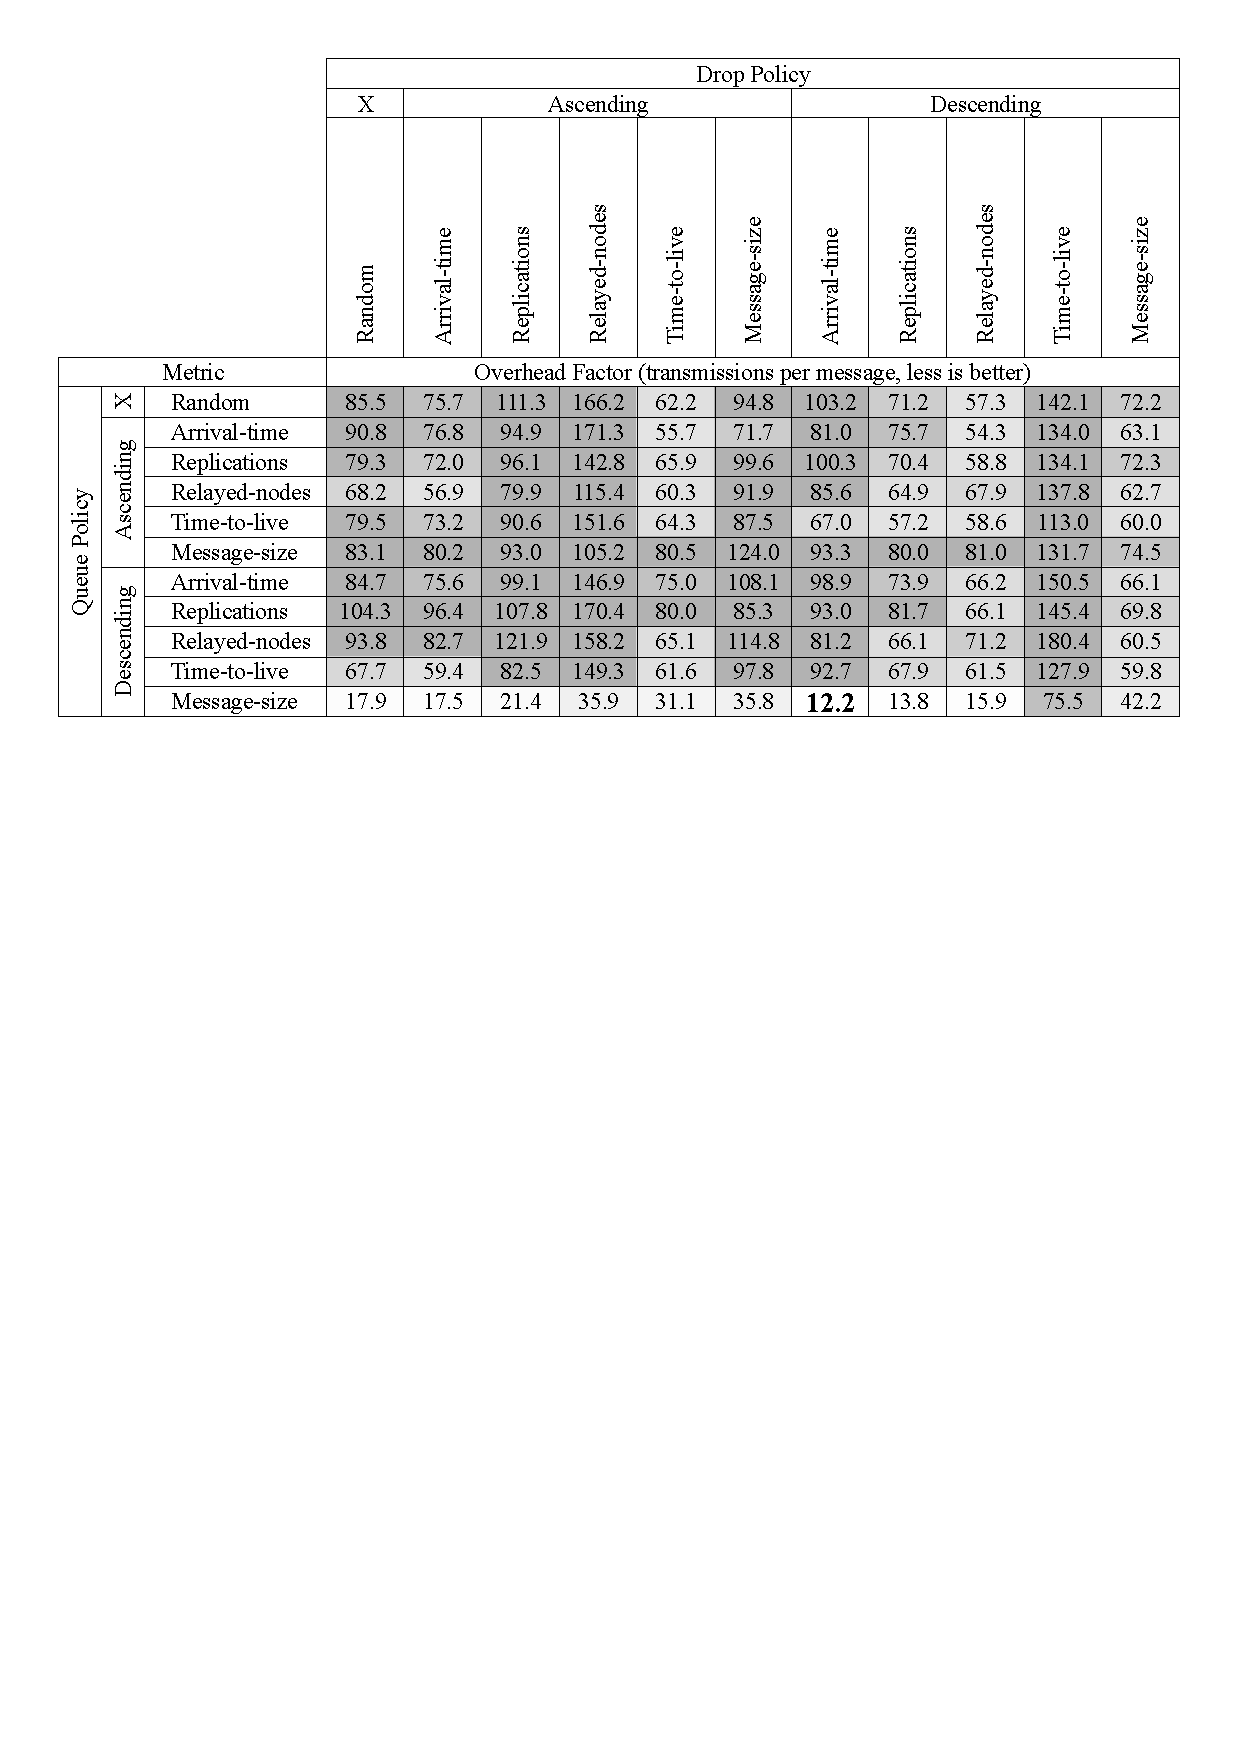
\includegraphics[width=1.0\textwidth]{fig/tables/scenario2_part2.pdf}
  \end{center}
\end{frame}

\begin{frame}
  \frametitle{Scenario 2 - Average Delay}
  \begin{center}
   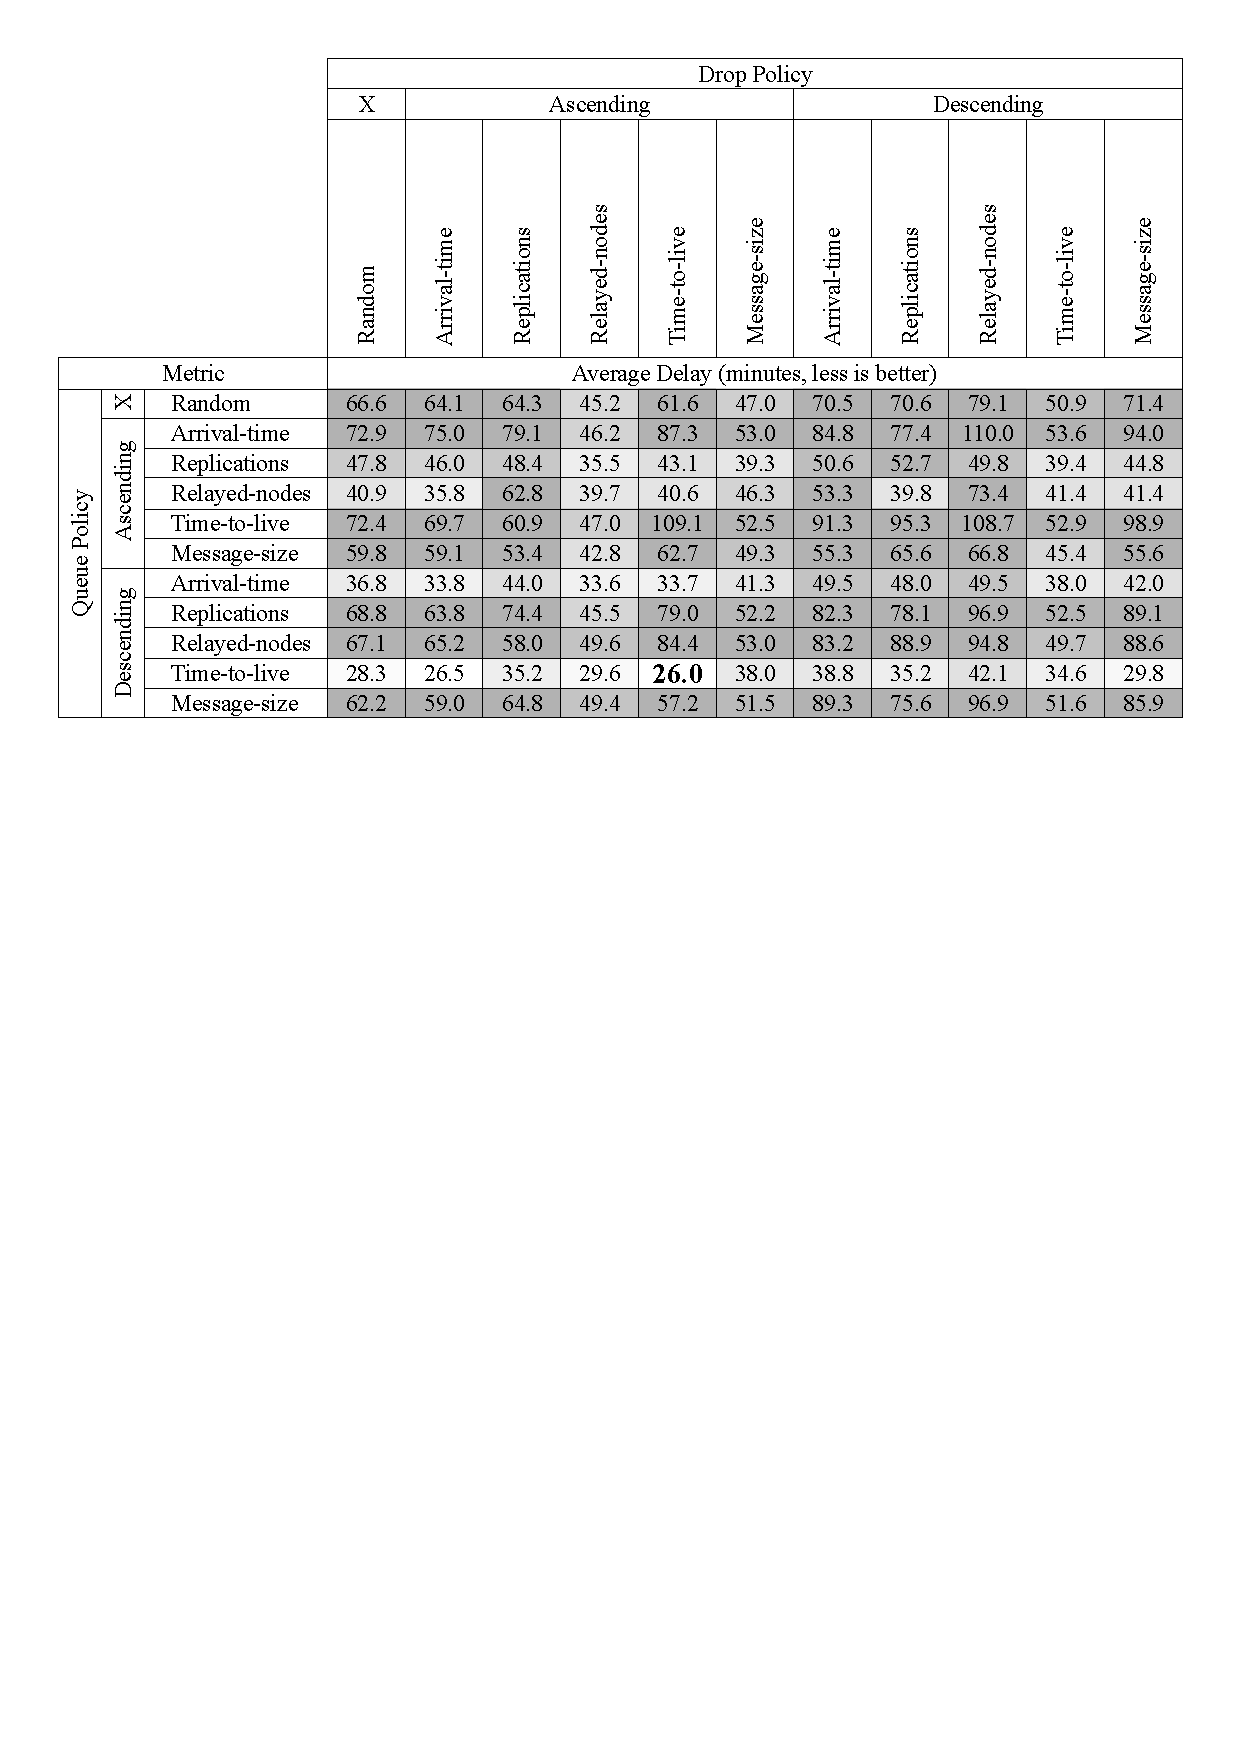
\includegraphics[width=1.0\textwidth]{fig/tables/scenario2_part3.pdf}
  \end{center}
\end{frame}

\begin{frame}
  \frametitle{Scenario 2 - Composite}
  \begin{center}
   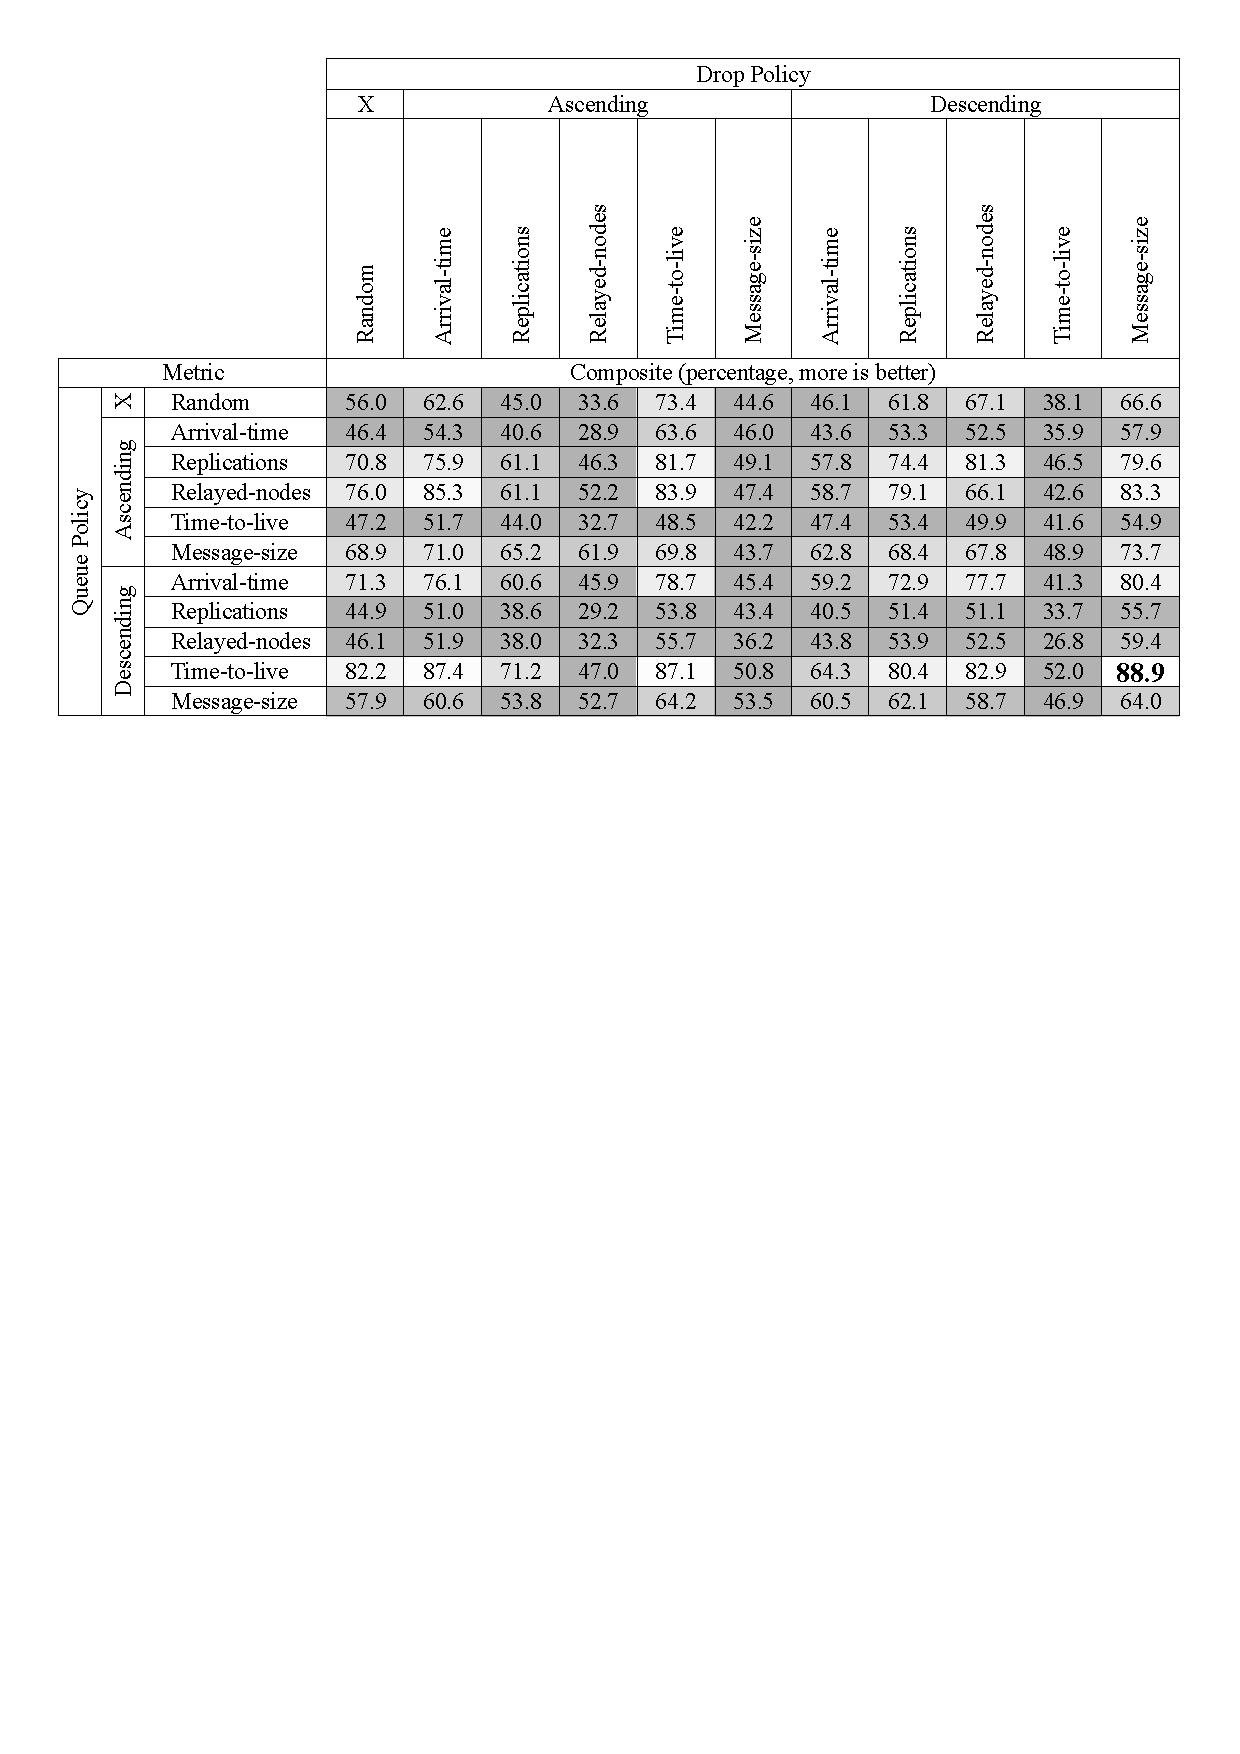
\includegraphics[width=1.0\textwidth]{fig/tables/scenario2_part4.pdf}
  \end{center}
\end{frame}

\end{document}


